\documentclass[journal]{IEEEtran}
\IEEEoverridecommandlockouts
\usepackage{array}
\usepackage{multirow}
\usepackage{graphicx}
\usepackage{textcomp}
\usepackage{xcolor}
\usepackage{tabularx,booktabs}
\newcolumntype{Y}{>{\centering\arraybackslash}X}
\newcolumntype{L}{>{\raggedright\arraybackslash}X}
\newcolumntype{P}[1]{>{\raggedright\arraybackslash}p{#1}}
\newcommand{\tablenote}[1]{\par\vspace{2pt}\begin{minipage}{0.98\linewidth}\footnotesize\raggedright #1\end{minipage}}
\usepackage{adjustbox}
% emergencystretch set by IEEEtran
\usepackage[english]{babel}
\setlength{\textfloatsep}{10pt plus 2pt minus 2pt}
\setlength{\floatsep}{8pt plus 2pt minus 2pt}
\setlength{\intextsep}{8pt plus 2pt minus 2pt}
\setlength{\tabcolsep}{4pt}
\renewcommand{\arraystretch}{1.08}
\raggedbottom
\setlength{\emergencystretch}{3em}

\usepackage{cite}
\usepackage{float}
\usepackage{amsmath,amssymb,amsfonts}
\usepackage{algorithm}
\usepackage{algpseudocode}
\usepackage{tikz}
\usepackage{placeins}
\usetikzlibrary{shapes.geometric, arrows.meta, positioning, chains, fit, backgrounds, decorations.pathreplacing}
\def\BibTeX{{\rm B\kern-.05em{\sc i\kern-.025em b}\kern-.08em
    T\kern-.1667em\lower.7ex\hbox{E}\kern-.125emX}}
% Load hyperref last so float and algorithm anchors are patched consistently.
\usepackage[hidelinks]{hyperref}
\hypersetup{
  pdftitle={BCHAIN-ACCESS: A Standards-Informed, Evidence-Aware Framework for Accessibility-Oriented Blockchain Healthcare Consent Interfaces},
  pdfauthor={Nadeem Yaqub and Muhammad Sami Ullah},
  pdfsubject={Accessibility-oriented blockchain healthcare consent interfaces},
  pdfkeywords={accessibility, blockchain, consent management, WCAG 2.2, design science research},
  pdfdisplaydoctitle=true,
  bookmarksopen=true,
  bookmarksnumbered=true,
  pdflang={en-US}
}

\begin{document}

\title{BCHAIN-ACCESS: A Standards-Informed, Evidence-Aware Framework for Accessibility-Oriented Blockchain Healthcare Consent Interfaces}

\author{Nadeem Yaqub and Muhammad Sami Ullah%
\thanks{Nadeem Yaqub is with the College of Computer Science and Technology, Beijing University of Technology, Beijing, China (e-mail: nadeem.yb@gmail.com).}%
\thanks{Muhammad Sami Ullah is with the Department of Computer Science, Gujrat Institute of Management Sciences (GIMS), an affiliated institute of PMAS-Arid Agriculture University Rawalpindi, Gujrat, Pakistan (e-mail: maliksami961@gmail.com).}}


\maketitle
% ============================================================
% ABSTRACT
% ============================================================
\begin{abstract}
Blockchain healthcare consent interfaces combine consequential authorization decisions with authentication, technical terminology, delayed transactions, and limited reversibility, creating accessibility risks that are not adequately represented in domain-specific design guidance. This paper presents BCHAIN-ACCESS, a standards-informed and evidence-aware framework developed through Design Science Research for accessibility-oriented blockchain healthcare consent interfaces. The framework connects twelve predicted accessibility-risk propositions to four design principles---Abstracted Authentication Design, Progressive Transparency Design, Confirmatory Interaction Design, and Assistive-Technology Compatibility---together with implementation responses, criterion-level WCAG~2.2 checks, and explicit evidence status. We operationalized the framework through a reference user-interface prototype and a separately tested local-EVM consent backend. Evaluation combined documentation-based evidence review, automated interface inspection, criterion-level expert review by ten domain experts who were not recruited as disabled end users, an expert task-based walkthrough, smart-contract testing, static analysis, and integration verification. Coarse heuristic ratings, perceived-usability scores, and custom questionnaire responses were also collected; because they were produced by unblinded non-target evaluators and, in the case of the heuristic ratings, cannot be shown to rest on independent observations, they are disclosed in the supplement and excluded from the reported results. Cycle~1 expert inspection identified actionable accessibility issues involving wizard-state announcements, contextual control names, and target size, while the mandatory confirmation wait emerged as a separate usability concern. A second design cycle addressed selected interface, contract, and backend issues identified in the first, and verified the refined artifact across 12 enumerated interface states, a 28-test Hardhat suite, and Slither static analysis. The final standalone axe-core reports recorded zero violations across the 12 tested states; five reports contained incomplete items retained for manual review. Added contract tests verified authorized audit logging and pause-policy enforcement, while API inspection verified single-record state-change handling. These results do not establish whole-artifact WCAG conformance, production security assurance, or accessibility effectiveness for disabled end users. BCHAIN-ACCESS contributes a reusable traceability structure for designing, implementing, and evaluating accessibility-oriented blockchain healthcare consent interfaces.
\end{abstract}
\begin{IEEEkeywords}
accessibility, blockchain, consent management, design science research, digital health, human--computer interaction, smart contracts, WCAG 2.2
\end{IEEEkeywords}
% ============================================================
% SECTION I: INTRODUCTION
% ============================================================
\section{Introduction}
Blockchain-mediated healthcare consent can provide verifiable authorization records, auditable permission changes, and patient-controlled access within a defined authorization model. However, the same systems expose users to unfamiliar authentication processes, technical terminology, delayed transaction states, and consequential actions that may be difficult to reverse. These interaction demands are especially important for users of assistive technologies and for people with visual, motor, cognitive, sensory, fatigue-related, temporary, or multiple access needs. Existing blockchain-healthcare research has primarily emphasized architecture, access control, integrity, and governance, while accessibility-oriented interface design and criterion-level evaluation remain comparatively underdeveloped \cite{tharani2022ui,khalid2023blockchain}. The accessibility work that does exist in this space targets general-purpose wallets rather than healthcare consent workflows \cite{zhou2023accessible}, and reports outcomes against assistive-technology use rather than tracing them to individual success criteria.

Prior blockchain HCI studies have examined application typologies, trust, wallet usability, health-record sharing, and dynamic consent \cite{elsden2018making,frohlich2022blockchain,zhou2023accessible,kim2022blockchain,khalid2023blockchain}. Closely related healthcare systems also address patient-controlled records and policy-based authorization \cite{dubovitskaya2020action,yaqub2025blockchain}. However, the reviewed work does not provide the same explicit end-to-end traceability from predicted accessibility risks to interface principles, implementation responses, criterion-level WCAG~2.2 checks, and evidence status. This missing traceability makes it difficult to determine which accessibility requirements have been implemented, simulated, technically tested, expert-inspected, remediated, or left for target-user confirmation.

This study addresses three research questions:

\noindent\textbf{RQ1:} What accessibility-related risks in blockchain healthcare consent interfaces are predicted by established accessibility standards, HCI principles, and closely related research?

\noindent\textbf{RQ2:} How can these predicted risks be translated into implementable accessibility-oriented design principles?

\noindent\textbf{RQ3:} How can a framework trace predicted risks to design obligations, implementation responses, criterion-level accessibility checks, and explicitly bounded evidence?

This paper makes five contributions:
\begin{enumerate}
\item \textbf{Predicted accessibility-risk propositions:} We formulate twelve standards-informed propositions covering authentication complexity, interface transparency, feedback adequacy, and assistive-technology compatibility.
\item \textbf{Accessibility-oriented design principles:} We translate these propositions into four implementable principles: Abstracted Authentication Design, Progressive Transparency Design, Confirmatory Interaction Design, and Assistive-Technology Compatibility.
\item \textbf{Evidence-aware traceability framework:} We introduce BCHAIN-ACCESS, which links each predicted risk to design obligations, implementation responses or statuses, criterion-level WCAG~2.2 checks, and the available evidence.
\item \textbf{Reference implementation:} We operationalize the framework through a user-interface prototype and a separately tested local-EVM consent backend implementing grant initiation, delayed confirmation, cancellation, revocation, and audit functions.
\item \textbf{Evaluation and Cycle~2 engineering evidence:} We provide Cycle~1 criterion-level expert findings and expert-identified interface issues, state-by-state browser and axe-core verification of the Cycle~2 interface, a 28-test smart-contract suite, Slither static analysis, and explicit evidence boundaries distinguishing Cycle~2 verification from target-user validation and production assurance. Expert measures that cannot be shown to rest on independent observations of the artifact by target users are disclosed in the supplement and excluded from the results.
\end{enumerate}

The distinctive contribution of BCHAIN-ACCESS is its evidence-aware traceability structure. Predicted accessibility risks are linked to design principles, implementation responses or statuses, criterion-level WCAG~2.2 checks, and the evidence available for each response. This structure distinguishes standards-derived requirements, implemented and simulated features, technically verified behavior, expert-identified issues, Cycle~2 refinement, unresolved risks, and elements requiring target-user confirmation. The contribution does not lie in proposing new accessibility standards; it lies in operationalizing existing accessibility and HCI requirements for blockchain-mediated healthcare consent.

The present study demonstrates framework operationalization, reference-artifact feasibility, and criterion-linked issue identification within the tested scope. The expert assessment is exploratory, and the implementation has not received production security, legal, or target-user effectiveness validation. Accordingly, the paper does not claim WCAG conformance or accessibility effectiveness for disabled end users.

The remainder of the paper is organized as follows. Section~II positions BCHAIN-ACCESS relative to blockchain healthcare, consent, HCI, and accessibility research. Section~III presents the Design Science Research methodology. Section~IV develops the predicted accessibility-risk propositions, and Section~V translates them into four design principles. Sections~VI and~VII present and operationalize the evidence-aware traceability framework. Section~VIII describes the reference implementation and technical verification, Section~IX reports the exploratory expert assessment, Section~X discusses implications and limitations, and Section~XI concludes.
% ============================================================
% SECTION II: BACKGROUND
% ============================================================
\section{Background}
\label{sec:background}

\subsection{Blockchain Technology in Healthcare}
Healthcare blockchain systems use smart contracts and replicated ledgers to coordinate authorization and record integrity, while clinical content is commonly kept off-chain \cite{kim2022blockchain,zhang2018fhirchain,dagher2018ancile}. This architecture can support traceability, but it does not make a system secure, private, or legally compliant by itself. Governance, controller and processor roles, necessity, data minimization, key management, identity assurance, biometric-data implications, and effective data-subject rights remain deployment-specific. Off-chain storage can reduce on-chain exposure but only partially mitigates rectification and erasure concerns, particularly where hashes or metadata remain personal data \cite{edpb2025blockchain}.

\subsection{Human-Computer Interaction and Accessibility}
WCAG~2.2 Level~A and~AA is the primary web-accessibility baseline in this study because SC~3.3.8 directly addresses accessible authentication \cite{wcag22}. WCAG conformance requires every applicable success criterion at the claimed level; automated scans and percentage scores cannot substitute for that determination. Nielsen's heuristics~\cite{nielsen1994usability,nielsen1992finding} are used as general usability prompts, not as disability-specific criteria; usability in the ISO~9241-11 sense \cite{iso9241} and accessibility conformance are treated as distinct properties throughout. Access needs are considered across visual, hearing, speech, motor and dexterity, cognitive and learning, fatigue-related, neurodivergent, temporary, and multiple-disability contexts \cite{who2023disability} rather than reduced to three homogeneous groups.

\subsection{Closest Related Work and Study Positioning}
Blockchain HCI research covers application typologies, trust, wallet usability, and interface design \cite{elsden2018making,frohlich2022blockchain,Glomann2019ImprovingTB,tharani2022ui}, including reviews of blockchain application interfaces \cite{tharatipyakul2021user}, ledger-client interface construction \cite{hossain2020designing}, and blockchain-mediated home health monitoring \cite{rahman2020natural}. Jang et al.~\cite{jang2020user} is a general DApp user-perspective study and is not treated here as healthcare-specific. The closest accessibility-specific work is Zhou et al.~\cite{zhou2023accessible}, who studied and iteratively redesigned a widely used non-custodial wallet with 44 participants, including 23 blind users, reporting accessibility failures against WCAG and measurable improvement across two design iterations. That work establishes wallet-level accessibility evidence with disabled participants; it does not address healthcare consent workflows, criterion-level traceability, or evidence-status reporting. It also supplies the class of target-user evidence that the present study explicitly does not provide (L2), and it is the model the evaluation proposed in Section~\ref{sec:future-work} should follow. Related consent-interface work outside blockchain includes Leimst\"adtner et al.~\cite{leimstadtner2024value}, who designed and evaluated a value-centered health data-sharing consent interface that uses reflective interface elements to counter heuristic disclosure decisions. Accessibility and disability considerations have also been raised in adjacent secured-assistant design \cite{alfayez2024user}. The closest healthcare work includes personal-health-record applications, patient-centric record sharing, policy-based access control, and dynamic consent for people with disabilities \cite{kim2022blockchain,dubovitskaya2020action,yaqub2025blockchain,khalid2023blockchain}. Blockchain-mediated medical data sharing \cite{taherdoost2023role} and blockchain-based dynamic consent for patient-centric research \cite{charles2024dynamic} provide the wider consent context. BCHAIN-ACCESS extends this work by making traceability from predicted accessibility risks to interface principles, implementation responses, criterion-level checks, and evidence status explicit. It does not claim to be the first framework to combine blockchain, consent, and disability-related concerns.

\begin{table*}[!htbp]
\centering
\small
\caption{Positioning relative to the closest blockchain healthcare and consent work}
\label{tab:related-comparison}
\begin{adjustbox}{max width=\textwidth,max totalheight=0.76\textheight,keepaspectratio}
\begin{tabular}{|p{3.3cm}|p{2.5cm}|p{2.7cm}|p{2.8cm}|p{3.2cm}|}
\hline
\textbf{Work} & \textbf{Primary focus} & \textbf{Accessibility treatment} & \textbf{Consent/access contribution} & \textbf{Distinction from this study} \\
\hline
Zhou et al.~\cite{zhou2023accessible} & Crypto-wallet accessibility & Evaluated with 23 blind users; WCAG failures reported & Not a consent framework & Provides target-user evidence this study lacks; does not address healthcare consent or criterion-level traceability \\
\hline
Khalid and Ahmed~\cite{khalid2023blockchain} & Dynamic consent and disability & Disability-oriented concept & Blockchain consent management & No explicit risk--principle--response--criterion--evidence traceability \\
\hline
Yaqub et al.~\cite{yaqub2025blockchain} & Healthcare access control & Not an interface evaluation & Policy-based authorization & This study focuses on interface traceability and expert inspection \\
\hline
Kim et al.~\cite{kim2022blockchain} & Personal health records & User experience, not WCAG conformance & Blockchain PHR application & This study adds standards-linked risk propositions \\
\hline
ACTION-EHR~\cite{dubovitskaya2020action} & Patient-centric cancer records & Not disability-specific & Patient-controlled record management & This study examines consent-interface accessibility \\
\hline
\textbf{BCHAIN-ACCESS} & Consent-interface design & Standards-informed and evidence-aware & Delayed confirmation and cancellable pending state & Risk--principle--response--criterion--evidence traceability supported by technical and exploratory expert evidence \\
\hline
\end{tabular}
\end{adjustbox}
\end{table*}

Yaqub et al.~\cite{yaqub2025blockchain} is prior work involving one of the present authors. It focuses on policy-based backend access control, whereas the present study focuses on standards-linked consent-interface propositions, traceability, reference implementation, and exploratory expert inspection.
% ============================================================
% SECTION III: METHODOLOGY
% ============================================================
\section{Methodology}
\label{sec:methodology}

We used Design Science Research (DSR) to connect problem evidence, artifact construction, and evaluation, drawing on established design-science guidance~\cite{hevner2004design} and adapting the six-activity DSRM process of Peffers et al.~\cite{peffers2007dsrm}: problem identification and motivation, definition of solution objectives, design and development, demonstration, evaluation, and communication. Table~\ref{tab:dsr-method} maps these activities into five study stages rather than treating framework construction and evaluation as results detached from method.

\begin{table*}[!htbp]
\centering
\small
\caption{Complete DSR methodology and evidence chain}
\label{tab:dsr-method}
\begin{tabularx}{\textwidth}{|p{2.2cm}|p{2.4cm}|X|p{2.4cm}|p{1.1cm}|p{2.2cm}|}
\hline
\textbf{Stage} & \textbf{Input} & \textbf{Procedure} & \textbf{Output} & \textbf{RQ} & \textbf{Evidence and involvement} \\
\hline
1. Problem identification and evidence gathering & Standards and prior blockchain, consent, accessibility, and HCI work & Targeted narrative synthesis and documentation review of three purposively selected systems & Evidence statements and predicted accessibility-risk propositions & RQ1 & Publications, whitepapers, product material, and prior reports; one literature screener and two document reviewers \\
\hline
2. Framework and principle derivation & Stage-1 propositions, WCAG~2.2 A/AA, Nielsen heuristics, and regulatory guidance & Trace each proposition to design obligations; synthesize and iteratively refine four principles and the framework & Risk--principle--response--criterion--evidence traceability model & RQ2--RQ3 & Standards and design rationale; author-led synthesis \\
\hline
3. Artifact design and implementation & Framework requirements and traceability model & Build the UI prototype and local-EVM reference backend; distinguish implemented, simulated, connected, and proposed elements & Reference implementation artifacts and testable interface states; the Cycle~1 build was not archived before refinement (L4) & RQ2--RQ3 & Source code, automated tests, and integration records; developer-researcher involvement \\
\hline
4. Expert feasibility evaluation & UI build, task script, criterion-level WCAG~2.2 checks, and heuristic instrument & Automated scans, criterion-level manual inspection, heuristic inspection, expert task-based walkthrough, SUS, and questionnaire & Tool findings, criterion-level manual findings, expert-identified issues, and quantitative measures later excluded (Section~\ref{sec:feasibility}) & RQ2--RQ3 & Ten domain experts not recruited as disabled end-user participants; exploratory, unblinded assessment \\
\hline
5. Cycle~2 refinement, final engineering verification, and synthesis & Outputs from Stages 1--4 and Cycle~2 source & Refine selected source issues; inspect enumerated browser states; run standalone axe-core, responsive and target-size checks, contract tests, Slither, and evidence-status synthesis without modifying the Cycle~1 findings & Cycle~2 artifact, final engineering evidence, updated statuses, residual risks, and future requirements & All & Researcher-led engineering verification; no disabled-participant or live screen-reader evidence \\
\hline
\end{tabularx}
\end{table*}

The adaptation maps problem identification to Stage~1, solution objectives to Stage~2, design and development to Stage~3, demonstration and evaluation to Stage~4, and refinement, final engineering verification, synthesis, and communication to Stage~5. The documentation review belongs to problem identification because it establishes what the public evidence does and does not substantiate and thereby motivates the risk propositions.

\subsection{Design Cycles and Artifact Provenance}
\label{subsec:cycles}

The reference artifact was developed over two design cycles, and this paper reports evidence from both. \textbf{Cycle~1} produced the initial prototype, which was the subject of the ten-expert assessment (Section~\ref{sec:feasibility}) and of the automated reports dated 29~June and 12~July 2026. \textbf{Cycle~2} refined that prototype in response to the Cycle~1 findings and produced the artifact verified on 15~July 2026 at commit \texttt{360eaa2a\allowbreak 26b2f2b4\allowbreak fef98c06\allowbreak 67f87db0\allowbreak 9e5e5120}. The accompanying working tree also contains a 19~July text-only consistency correction that changes the review-screen duration from an unsupported ``30 days'' to the gateway's actual no-expiry default; no Cycle~1 finding or 15~July automated result is attributed to that later edit. Iterating between build and evaluation is the expected DSR pattern~\cite{peffers2007dsrm,hevner2004design}; the two cycles are named here so that every result in this paper can be attributed to the artifact it was obtained from.


\begin{figure*}[!t]
\centering
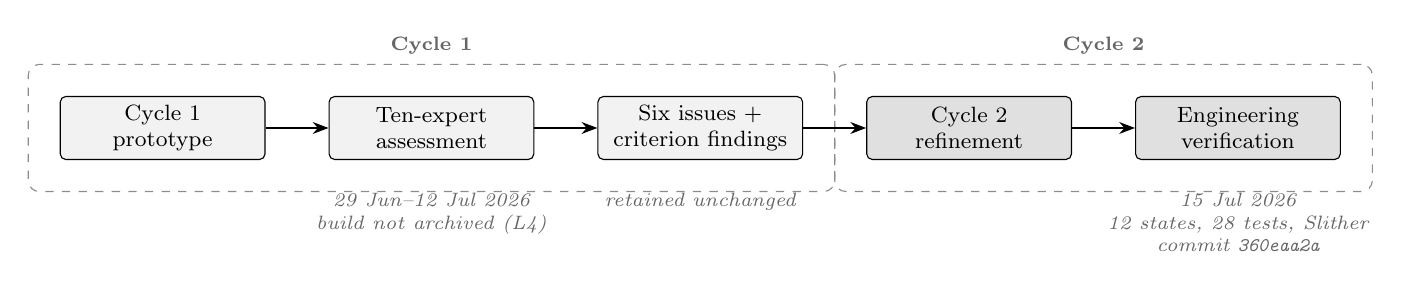
\begin{tikzpicture}[
  font=\footnotesize,
  box/.style={draw, rounded corners=2pt, minimum height=8mm, minimum width=26mm, align=center, inner sep=2pt},
  c1/.style={box, fill=black!5},
  c2/.style={box, fill=black!12},
  ar/.style={-{Stealth[length=2mm]}, thick},
  note/.style={font=\scriptsize\itshape, text=black!60, align=center}
]
\node[c1] (build1) {Cycle~1\\prototype};
\node[c1, right=8mm of build1] (eval1) {Ten-expert\\assessment};
\node[c1, right=8mm of eval1] (find) {Six issues~+\\criterion findings};
\node[c2, right=8mm of find] (build2) {Cycle~2\\refinement};
\node[c2, right=8mm of build2] (ver) {Engineering\\verification};
\draw[ar] (build1) -- (eval1);
\draw[ar] (eval1) -- (find);
\draw[ar] (find) -- (build2);
\draw[ar] (build2) -- (ver);
\node[note, below=3mm of eval1] {29~Jun--12~Jul 2026\\build not archived (L4)};
\node[note, below=3mm of ver] {15~Jul 2026\\12 states, 28 tests, Slither\\commit \texttt{360eaa2a}};
\node[note, below=3mm of find] {retained unchanged};
\begin{scope}[on background layer]
\node[draw, dashed, black!45, rounded corners, fit=(build1)(eval1)(find), inner sep=4mm,
      label={[font=\scriptsize\bfseries, text=black!60]above:Cycle~1}] {};
\node[draw, dashed, black!45, rounded corners, fit=(build2)(ver), inner sep=4mm,
      label={[font=\scriptsize\bfseries, text=black!60]above:Cycle~2}] {};
\end{scope}
\end{tikzpicture}
\caption{Evidence provenance across the two design cycles. The expert-assessed Cycle~1 build was not archived before refinement (L4). Cycle~2 produced the verified build, while Cycle~1 findings remain unchanged.}
\label{fig:cycles}
\end{figure*}

Fig.~\ref{fig:cycles} summarizes the two cycles and the evidence each produced. Cycle~2 corrected selected interface, contract, and backend issues identified in Cycle~1, and the resulting build was examined through state-by-state axe-core scans, manual browser and keyboard checks, rendered target measurements, responsive inspection, Hardhat testing, and Slither static analysis. Evidence is reported against the cycle that produced it: Cycle~1 findings are not revised by Cycle~2 changes, and no Cycle~2 result is used to characterize the Cycle~1 artifact. The Cycle~1 build was not archived before refinement; the consequences are stated once in Limitation~L4 and the retained metadata is listed in Supplementary~S9.2. Evaluation with participants recruited as disabled end users remains future work for both cycles.

\subsection{Stage 1: Problem Identification and Evidence Gathering}
A targeted narrative synthesis was used to identify relevant blockchain-healthcare, consent, HCI, and accessibility work and to motivate the initial barrier propositions. It supported problem formulation and contribution positioning and was not intended as an exhaustive or systematic review. Sources searched, relevance reasoning, and exclusions are recorded in Supplementary~S7.

\subsection{Stage 1b: Documentation-Based Evidence Review}
\label{subsec:heuristic-eval}
We selected three systems through purposive maximum-variation sampling to identify documented interface concerns. The goal was a structured documentation-based evidence review of publicly available interface material, prioritizing analytical depth over statistical generalization, rather than hands-on heuristic evaluation of live systems. MedRec~\cite{medrec} (academic prototype), Patientory (commercial patient-engagement platform), and BurstIQ (enterprise health-data marketplace) were selected because they represent three widely cited architectural paradigms in blockchain healthcare, providing maximum architectural variation while spanning the deployment spectrum. They are also among the few blockchain healthcare systems with sufficient public interface documentation to support concern identification.

Because the review used documents rather than live systems, it cannot establish frequency, task impact, persistence, or inability to complete a task. Nielsen ratings are retained only as concern prompts and are not interpreted as observed severity. Apparent recurrence means recurrence in the reviewed evidence corpus, not demonstrated recurrence in the products.

The review used Nielsen's heuristics~\cite{nielsen1994usability} as analytic prompts and selected WCAG~2.2 A/AA success criteria as an evidence-coding frame. Heuristic inspection has been applied to accessibility evaluation before, but its coverage of disability-specific criteria is partial \cite{paz2019heuristic}, which is why heuristics are not used here as accessibility criteria. Because documentation cannot demonstrate live conformance, reviewers coded each item as \emph{Evidenced}, \emph{Partially evidenced}, \emph{Not evidenced}, or \emph{Not assessable}. ``Not evidenced'' means only that the reviewed corpus did not substantiate the feature; it is not a failure judgment. A failure is reported only where a source provides direct evidence of non-conformance. SC~3.1.5 (Reading Level) is Level~AAA and is therefore excluded from the A/AA set; plain-language observations are retained as non-conformance-neutral design evidence.

The documentation-based evidence review was coded independently by two reviewers using published interface documentation, user reviews, and prior usability study reports.\footnote{Primary sources per system: MedRec, original conference paper~\cite{medrec} and MIT Media Lab interface specification; Patientory, official whitepaper (v2.0, 2022) and App/Play Store reviews (2022--2024); BurstIQ, product documentation portal (accessed 2024) and usability data reported in prior work.} Inter-rater disagreements were resolved through discussion and consensus. Results are reported in Section~\ref{sec:barriers}.

Both reviewers hold postgraduate HCI qualifications and at least three years of usability-inspection experience. The previously reported pooled Cohen's $\kappa=0.74$ combined unlike ordinal and categorical scales and is withdrawn. Because the surviving source package does not contain the separate pre-consensus contingency tables needed to recompute weighted ordinal and categorical agreement, no baseline reliability coefficient is claimed. Consensus evidence codes are reported descriptively, and this missing provenance is a limitation.

\subsection{Stages 2--5: Derivation, Construction, Evaluation, and Analysis}
Stage~2 translated each predicted accessibility-risk proposition into a standards-linked design obligation and iteratively grouped those obligations into the four principles and framework described in Sections~\ref{sec:principles} and~\ref{sec:framework}. Stage~3 implemented a UI prototype and a separate local-EVM backend, with artifact boundaries and implementation status reported in Section~\ref{sec:implementation}. Stage~4 evaluated the UI through automated scans and an exploratory expert feasibility inspection; integration tests evaluated the connected build separately. Stage~5 triangulated automated, manual, and qualitative evidence, refined selected source issues in Cycle~2, and added a separately reported engineering-verification layer, with manual findings taking precedence over aggregate coverage indicators. The quantitative expert measures were excluded at this stage for the reasons given in Section~\ref{sec:feasibility}.
% ============================================================
% SECTION IV: BARRIERS
% ============================================================
\section{Predicted Accessibility-Risk Propositions}
\label{sec:barriers}

This section addresses \textbf{RQ1} by presenting twelve standards-informed accessibility-risk propositions organized across four dimensions: authentication complexity, interface transparency, feedback adequacy, and assistive-technology compatibility. The propositions synthesize requirements and concerns derived from WCAG~2.2, Nielsen's heuristics, closely related research, and the documentation-based evidence review and identify design risks requiring implementation and evaluation attention.

\subsection{Risk-Proposition Taxonomy}

\noindent\textbf{Dimension~1: Authentication Complexity.}\ Direct interaction with cryptographic credentials may create cognitive, visual, and motor demands. SC~3.3.8 requires an accessible authentication path without a cognitive-function test unless an allowed mechanism is provided \cite{wcag22}.

\textbf{B1, Key Management Burden:} Direct key generation, storage, recovery, or entry may create memory, comprehension, vision, and dexterity barriers when required by an implementation. Wallet studies report exactly these burdens for blind users \cite{zhou2023accessible}, and alias mechanisms have been proposed to reduce raw-address handling \cite{bodziony2021blockchain}.

\textbf{B2, Authentication Complexity:} Multi-step authentication may create barriers. Where an authentication workflow imposes a user-completion deadline, SC~2.2.1 requires the applicable timing protections; cognitive-function tests require accessible alternatives under SC~3.3.8.

\textbf{B3, Authentication Alternatives Not Evidenced:} The reviewed documents did not substantiate accessible alternatives. This is an evidence gap, not proof that the products lack them.

\noindent\textbf{Dimension~2: Interface Transparency.}\ Blockchain's underlying processes---transaction verification, consensus, and block confirmation---are invisible to users yet directly affect system responsiveness \cite{frohlich2022blockchain}.

\textbf{B4, Unclear System Status:} Delayed transaction states may be difficult to interpret when interfaces do not expose pending, confirmed, failed, and retry states in perceivable language.

\textbf{B5, Technical Language:} Unexplained terms such as ``gas'', ``wallet address'', and ``hash'' may increase cognitive load. Plain language is a design recommendation; SC~3.1.5 is Level~AAA and is not counted in the A/AA instrument.

\textbf{B6, Opaque Data and Permission Representation:} Users may be unable to determine storage location, active permissions, and access history when these are not presented explicitly. This is relevant to transparency but does not establish GDPR compliance or non-compliance~\cite{gdpr2016}.

\noindent\textbf{Dimension~3: Feedback Adequacy.}\ Effective feedback is a foundational HCI requirement, particularly critical in healthcare contexts where incorrect actions may have clinical consequences \cite{tharani2022ui}.

\textbf{B7, Non-Actionable Errors:} Raw system messages may not identify an error or explain recovery in terms users can act on (SC~3.3.1 and Nielsen H9).

\textbf{B8, Inadequate Confirmation Feedback:} Consequential consent actions require perceivable confirmation and a clear distinction between queued and finalized states.

\textbf{B9, Limited Reversal:} Some finalized ledger actions cannot be deleted or technically reversed. Interfaces should prevent errors and explain compensating actions such as revocation; documentary absence of warnings is not treated as a demonstrated product failure.

\noindent\textbf{Dimension~4: Assistive-Technology Compatibility.}\ Compatibility must be evaluated for the technologies, input modes, and interface states in scope; no design can claim universal compatibility from standards inspection alone.

\textbf{B10, Dynamic-Update Announcement Risk:} Transaction and wizard-state changes may be missed when programmatic status semantics are absent or incomplete (SC~4.1.3).

\textbf{B11, Input Operability and Target-Size Risk:} Wallet and consent workflows may exclude keyboard or alternative-input users when operability, focus order, focus visibility, and target size are not implemented and tested (SC~2.1.1, SC~2.4.3, SC~2.4.7, and SC~2.5.8). Switch and voice-input compatibility were not tested in this study.

\textbf{B12, Visual Distinguishability Risk:} Text, controls, focus indicators, and status cues require measured text and non-text contrast and non-color alternatives (SC~1.4.3 and SC~1.4.11). The reviewed documents did not contain sufficient evidence for product-level contrast judgments.

\subsection{Access-Need Relevance Mapping}

Table~\ref{tab:barrier-disability} provides an illustrative design-aid mapping between the twelve risk propositions and three access-need clusters most directly represented in the present framework: cognitive and learning, visual, and motor and dexterity needs. The mapping records author-identified potential relevance rather than participant evidence and is not intended as a comprehensive disability taxonomy. Hearing, speech, fatigue-related, neurodivergent, temporary, and multiple-disability contexts require subsequent refinement through co-design and target-user evaluation.

\begin{table*}[!t]
\centering
\small
\caption{Illustrative Risk-Proposition to Access-Need Mapping}
\label{tab:barrier-disability}
\begin{adjustbox}{max width=\textwidth,keepaspectratio}
\begin{tabular}{|p{2.8cm}|*{12}{c|}}
\hline
\textbf{Access-need cluster} & \textbf{B1} & \textbf{B2} & \textbf{B3} & \textbf{B4} & \textbf{B5} & \textbf{B6} & \textbf{B7} & \textbf{B8} & \textbf{B9} & \textbf{B10} & \textbf{B11} & \textbf{B12} \\
\hline
Cognitive and learning & $\bullet$ & $\bullet$ &  & $\bullet$ & $\bullet$ & $\bullet$ & $\bullet$ & $\bullet$ & $\bullet$ &  &  &  \\
\hline
Visual & $\bullet$ &  & $\bullet$ &  &  & $\bullet$ &  &  &  & $\bullet$ & $\bullet$ & $\bullet$ \\
\hline
Motor and dexterity & $\bullet$ & $\bullet$ &  &  &  &  &  &  &  &  & $\bullet$ &  \\
\hline
\multicolumn{13}{l}{\footnotesize\textit{Note.} $\bullet$ indicates potential relevance identified by the authors for design and evaluation planning, except B1$\times$Visual,}\\
\multicolumn{13}{l}{\footnotesize which is supported by reported wallet-accessibility findings with blind users~\cite{zhou2023accessible}. Otherwise it does not represent participant-confirmed impact.}\\
\end{tabular}
\end{adjustbox}
\end{table*}

\subsection{Documentation-Based Evidence Summary}

The documentation review recorded heuristic concerns and selected WCAG~2.2 interface patterns using the evidence categories defined in Section~\ref{subsec:heuristic-eval}. The complete heuristic evidence matrix is provided in Supplementary~S8.1. Table~\ref{tab:wcag-documentation} retains the criterion-level summary most directly relevant to framework derivation.

\begin{table}[H]
\caption{Documentation Evidence for Selected WCAG~2.2 A/AA Interface Patterns}
\label{tab:wcag-documentation}
\centering
\scriptsize
\renewcommand{\arraystretch}{1.08}
\setlength{\tabcolsep}{2pt}
\begin{tabularx}{\linewidth}{|L|Y|Y|Y|>{\centering\arraybackslash}p{0.10\linewidth}|}
\hline
\textbf{WCAG Criterion} & \textbf{MedRec} & \textbf{Patientory} & \textbf{BurstIQ} & \textbf{Risk} \\
\hline
1.4.3 Color Contrast & Not assessable & Not assessable & Not assessable & B12 \\
\hline
1.4.11 Non-text Contrast & Not assessable & Not assessable & Not assessable & B12 \\
\hline
2.1.1 Keyboard Access & Not assessable & Partially evidenced & Not assessable & B11 \\
\hline
2.4.3 Focus Order & Not assessable & Not assessable & Not assessable & B11 \\
\hline
2.2.1 Timing Adjustable & Not evidenced & Partially evidenced & Not evidenced & B2 \\
\hline
2.4.7 Focus Visible & Not assessable & Evidenced & Partially evidenced & B11 \\
\hline
2.5.8 Target Size (Minimum) & Not assessable & Not assessable & Not assessable & B11 \\
\hline
3.3.1 Error Identification & Not evidenced & Partially evidenced & Not evidenced & B7 \\
\hline
3.3.2 Labels \& Instructions & Not evidenced & Evidenced & Partially evidenced & B7 \\
\hline
3.3.4 Error Prevention (Data) & Not evidenced & Not evidenced & Not evidenced & B8, B9 \\
\hline
3.3.8 Accessible Authentication & Not evidenced & Not evidenced & Not evidenced & B1--B3 \\
\hline
4.1.3 Status Messages & Not assessable & Not assessable & Not assessable & B10 \\
\hline
\end{tabularx}
\vspace{2pt}
\parbox{\linewidth}{\footnotesize\textit{Note.} ``Not evidenced'' means the reviewed corpus did not substantiate the pattern; ``Not assessable'' means documents could not support a judgment. SC~3.1.5 is excluded because it is Level~AAA. No aggregate score is calculated for documentary evidence.}
\end{table}

\subsection{Resulting Design Obligations}
\label{sec:gap-analysis}
The documentation review showed uneven and frequently insufficient public evidence for accessibility-related interface patterns across the three illustrative systems. In BCHAIN-ACCESS, these findings motivate twelve inspectable design propositions. Each proposition is translated in Section~V into a design obligation and is subsequently connected to an implementation response, criterion-level check, and evidence status.
% ============================================================
% SECTION V: HCI PRINCIPLES
% ============================================================
\section{Accessibility-Oriented Design Principles}
\label{sec:principles}

This section addresses \textbf{RQ2} by translating the twelve predicted accessibility-risk propositions into four implementable and inspectable design principles: Abstracted Authentication Design (AAD), Progressive Transparency Design (PTD), Confirmatory Interaction Design (CID), and Assistive-Technology Compatibility (ATC). Together, the principles organize authentication, transparency, feedback, and assistive-technology obligations and connect them to prototype responses and criterion-level accessibility checks.

The principles were derived deductively from the risk propositions and their standards basis, forming an author-designed structure for organizing traceable design obligations.

\subsection{Principle 1: Abstracted Authentication Design (AAD)}

Cryptographic authentication demands should be minimized or mediated through accessible mechanisms that do not require users to manipulate raw credentials directly. Secure hardware, biometrics, and representative access are production recommendations not implemented in this reference artifact. Any delegation model requires jurisdiction-specific authority, scope, expiry, revocation, representative identification, abuse safeguards, and distinct audit records. Authentication time limits must follow SC~2.2.1 by allowing users to turn off, adjust, or extend the limit unless a stated exception applies; the criterion does not require a 20-hour session option.

\subsection{Principle 2: Progressive Transparency Design (PTD)}

Blockchain states should be disclosed progressively in actionable language. Technical terms should be explained inline and through a glossary; this is advisory plain-language guidance, not a Level~AA claim under SC~3.1.5, which is Level~AAA. Storage status, permissions, and access history should be perceivable, while any legal-transparency conclusion requires separate assessment.

\subsection{Principle 3: Confirmatory Interaction Design (CID)}

Consequential consent actions should provide an explicit review stage, a plain-language statement of consequences, and a recoverable checkpoint before finalization. The reference contract implements a two-stage delayed-confirmation state machine with cancellation available until confirmation. Its reference configuration uses a 60-second minimum waiting period. Interface elements that deliberately slow a consequential disclosure decision to encourage reflection have been designed and evaluated with patients in health data-sharing consent \cite{leimstadtner2024value}, which supports the mechanism in principle. The waiting period may reduce accidental or impulsive activation, but its duration remains empirically unresolved and it does not prevent coercion. Error states should identify the problem and provide an actionable recovery path (SC~3.3.1).

\subsection{Principle 4: Assistive-Technology Compatibility (ATC)}

Interfaces should be tested with the assistive technologies and input modes in the stated scope. Dynamic updates require appropriate programmatic status semantics (SC~4.1.3); workflows require keyboard, focus-order, focus-visibility, and target-size testing (SC~2.1.1, SC~2.4.3, SC~2.4.7, and SC~2.5.8); and visual presentation requires text and non-text contrast checks (SC~1.4.3 and SC~1.4.11). Compatibility claims must remain limited to the technologies, configurations, and interface states actually tested.

Table~\ref{tab:principles} summarizes the mapping between principles, risk propositions, and standards.

\begin{table}[!htbp]
\caption{Design Principles Mapped to Risk Propositions and Standards}
\label{tab:principles}
\centering
\small
\renewcommand{\arraystretch}{1.12}
\begin{tabularx}{\linewidth}{|Y|Y|Y|L|}
\hline
\textbf{Principle} & \textbf{Risk Propositions} & \textbf{Nielsen} & \textbf{WCAG 2.2} \\
\hline
AAD & B1, B2, B3 & H5, H6 & 2.2.1, 3.3.8$^{\ddagger}$ \\
\hline
PTD & B4, B5, B6 & H1, H2 & 3.3.2, 4.1.3$^{\S}$; 3.1.3, 3.1.5 (AAA) \\
\hline
CID & B7, B8, B9 & H3, H5, H9 & 3.3.1, 3.3.2, 3.3.4 \\
\hline
ATC & B10, B11, B12 & H4, H7 & 1.4.3, 1.4.11, 2.1.1, 2.4.3, 2.4.7, 2.5.8, 4.1.3 \\
\hline
\end{tabularx}
\tablenote{$^{\ddagger}$SC~3.3.8 (Accessible Authentication) is central to AAD. Representative access is a framework recommendation and is not implemented. For PTD, SC~3.1.3 (Unusual Words) and SC~3.1.5 (Reading Level) are Level~AAA/advisory references; plain-language and jargon-reduction guidance does not constitute a Level~A/AA conformance claim. $^{\S}$SC~4.1.3 (Status Messages) is shared by PTD and ATC: PTD governs whether the status content is expressed in perceivable, actionable language (B4), whereas ATC governs whether the status change is exposed programmatically (B10).}
\end{table}

\subsection{Illustrative Traceability Example}

Consider a hypothetical patient granting a neurologist temporary access to an MRI record. The workflow illustrates how AAD reduces direct credential-management demands, PTD presents permissions and transaction states in actionable language, CID provides review and cancellable confirmation, and ATC requires keyboard, focus, status-announcement, contrast, and target-size inspection. The expert task workflow is reported in Section~IX, and the complete workflow-to-principle mapping is provided in Supplementary~S8.7.
% ============================================================
% SECTION VI: THE BCHAIN-ACCESS FRAMEWORK (RQ3)
% ============================================================
\section{The BCHAIN-ACCESS Evidence-Aware Framework}
\label{sec:framework}

This section addresses \textbf{RQ3} by integrating the four design principles into an evidence-aware framework for accessibility-oriented blockchain healthcare consent interfaces. BCHAIN-ACCESS combines healthcare, blockchain, governance and regulation, and HCI and accessibility perspectives; makes explicit the design obligations arising at their intersections; and traces each predicted risk to an implementation response or status, criterion-level check, and evidence status.

The framework distinguishes what is standards-derived, implemented, simulated, technically verified, expert-inspected, remediated, unresolved, or reserved for target-user confirmation. These evidence statuses make the support for each response and the remaining work directly inspectable.

\subsection{Four Design Perspectives}

BCHAIN-ACCESS treats an accessibility-oriented blockchain healthcare consent interface as the joint product of four perspectives, each contributing a distinct class of design obligations.

\noindent\textbf{P1, Healthcare Perspective.}\ The setting is patient-controlled
consent management for electronic health records within a multi-provider care
network, where an incorrect action can carry clinical consequences
(Section~\ref{sec:background}). This perspective supplies the workflow the framework
must serve, patient-controlled consent within the modeled authorization scope, provider access grants, and an auditable
consent history, illustrated by the traceability example in Section~V. Patient perspectives on health-data sharing motivate treating consent comprehension as a design requirement rather than a formality \cite{magsamen2019patient}.

\noindent\textbf{P2, Blockchain Perspective.}\ The intended architecture stores clinical content off-chain and records identifiers or digests on-chain. The reference backend demonstrates consent-state transitions using seeded 32-byte identifiers; it does not implement a production off-chain clinical-record repository. The intended deployment setting is a permissioned consortium network; the consensus mechanism is deployment-specific and was not evaluated in the reference artifact (Section~\ref{subsec:blockchain-architecture}). Conceptual scope distinctions relative to centralized-EHR and pure-Ethereum architecture patterns are summarized in Supplementary~S3; they are category-level distinctions rather than empirical comparisons against evaluated systems.

\noindent\textbf{P3, Governance and Regulation Perspective.}
The framework records GDPR Articles~6, 13, and~17~\cite{gdpr2016}, EN~301~549~\cite{en301549}, Section~508~\cite{section508}, and, where relevant, HIPAA~\cite{hipaa1996} as deployment-specific regulatory and governance considerations. These sources inform design questions concerning lawful basis, transparency, data-subject rights, institutional roles, privacy engineering, and accessibility procurement. BCHAIN-ACCESS does not determine legal compliance. Off-chain storage with on-chain digest references can reduce direct on-chain exposure but does not by itself resolve erasure, rectification, controller responsibility, or metadata-identifiability concerns.

\noindent\textbf{P4, HCI and Accessibility Perspective.}\ Accessibility is required
through criterion-level WCAG~2.2 and heuristic inspection, operationalized as
the four principles AAD, PTD, CID, and ATC (Section~\ref{sec:principles}). People with
disabilities are the framework's primary intended beneficiaries.

\subsection{Cross-Perspective Design Obligations}

A central design premise of BCHAIN-ACCESS is that several consequential problems arise at the intersections of perspectives, where satisfying one concern can introduce risks for another. The framework makes these obligations explicit rather than leaving them to be discovered during implementation. Fig.~\ref{fig:perspectives} shows the four perspectives, the tension each pairing creates, and the design response that discharges it.

\begin{figure*}[!t]
\centering
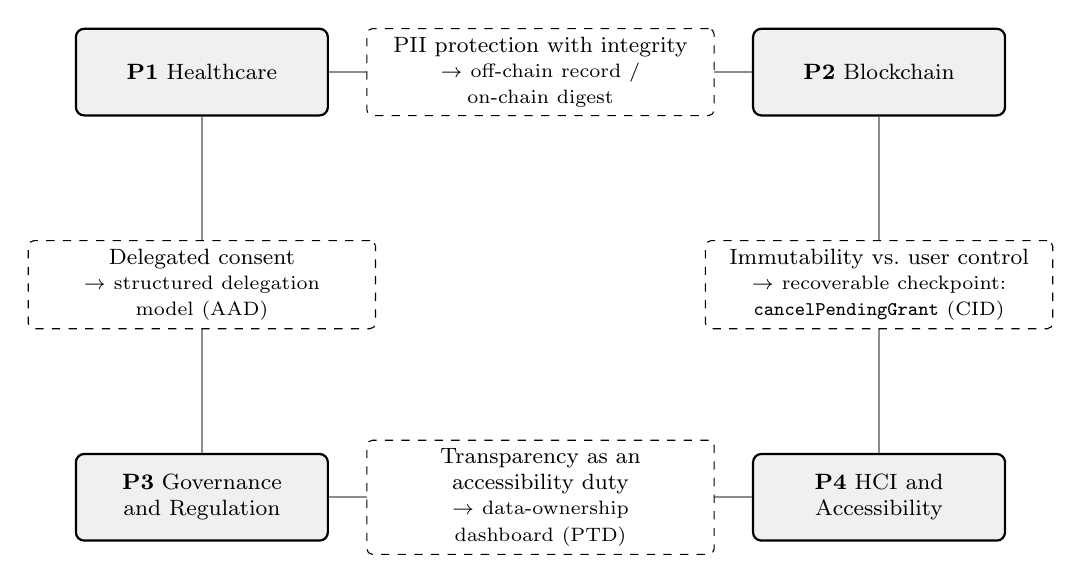
\begin{tikzpicture}[
  font=\footnotesize,
  persp/.style={draw, thick, rounded corners=3pt, minimum height=11mm, minimum width=32mm,
                align=center, fill=black!6, inner sep=3pt},
  obl/.style={draw, dashed, rounded corners=2pt, align=center, inner sep=3pt,
              fill=white, text width=42mm},
  link/.style={-, thick, black!45}
]
\node[persp] (p1) at (0,0)      {\textbf{P1} Healthcare};
\node[persp] (p2) at (8.6,0)    {\textbf{P2} Blockchain};
\node[persp] (p3) at (0,-5.4)   {\textbf{P3} Governance\\and Regulation};
\node[persp] (p4) at (8.6,-5.4) {\textbf{P4} HCI and\\Accessibility};
\draw[link] (p1) -- (p2);
\draw[link] (p1) -- (p3);
\draw[link] (p2) -- (p4);
\draw[link] (p3) -- (p4);
\node[obl] at (4.3,0)    {PII protection with integrity\\[1pt]{\scriptsize$\rightarrow$ off-chain record /\\on-chain digest}};
\node[obl] at (0,-2.7)   {Delegated consent\\[1pt]{\scriptsize$\rightarrow$ structured delegation\\model (AAD)}};
\node[obl] at (8.6,-2.7) {Immutability vs.\ user control\\[1pt]{\scriptsize$\rightarrow$ recoverable checkpoint:\\\texttt{cancelPendingGrant} (CID)}};
\node[obl] at (4.3,-5.4) {Transparency as an\\accessibility duty\\[1pt]{\scriptsize$\rightarrow$ data-ownership\\dashboard (PTD)}};
\end{tikzpicture}
\caption{The four BCHAIN-ACCESS design perspectives and the obligations arising at their intersections. Each obligation is generated by a tension between two perspectives and is discharged by a specific design response, shown after the arrow. These are the intersections the framework develops; they are not claimed to exhaust the possible pairings.}
\label{fig:perspectives}
\end{figure*}


\noindent\textbf{Blockchain~$\times$~HCI, immutability versus user control.}\
Blockchain's immutability constrains the undo and recovery pathways associated with Nielsen's H3 and H9. The documentation review identified this as a recurring design concern, but it did not measure live-system severity or task impact (Section~\ref{sec:gap-analysis}). The obligation is a
recoverable-checkpoint mechanism that preserves ledger integrity: the CID time-locked
consent pending state (\texttt{cancelPendingGrant}).

\noindent\textbf{Governance~$\times$~HCI, transparency as an accessibility duty.}\
The GDPR Article~13 transparency requirement~\cite{gdpr2016} and Nielsen's visibility heuristic (H1)
are jointly served by the PTD data-ownership dashboard, which presents on-chain versus
off-chain status, active consent permissions, and access logs in screen-reader-
compatible plain language.

\noindent\textbf{Healthcare~$\times$~Blockchain, PII protection with integrity.}\
Protecting patient PII while retaining tamper-evidence obliges the off-chain-record /
on-chain-digest pattern. Per-record salting is a production recommendation; the reference backend uses deterministic seeded identifiers and does not implement a salt store.

\noindent\textbf{Healthcare~$\times$~Governance, delegated consent.}\ Care contexts
in which a patient cannot self-authenticate oblige a structured delegation model in
which a trusted guardian or authorized representative acts under an auditable on-chain
consent record, subject to jurisdiction-specific rules governing legal representation,
capacity, authorization, lawful basis, and healthcare consent (Principle~AAD).

Because these obligations are defined at perspective intersections rather than within a
single concern, they distinguish BCHAIN-ACCESS from prior frameworks that treat
healthcare, blockchain, governance, and HCI as independent
concerns~\cite{khalid2023blockchain,tharani2022ui}.

\subsection{Risk-to-Evidence Traceability}


\begin{figure*}[!t]
\centering
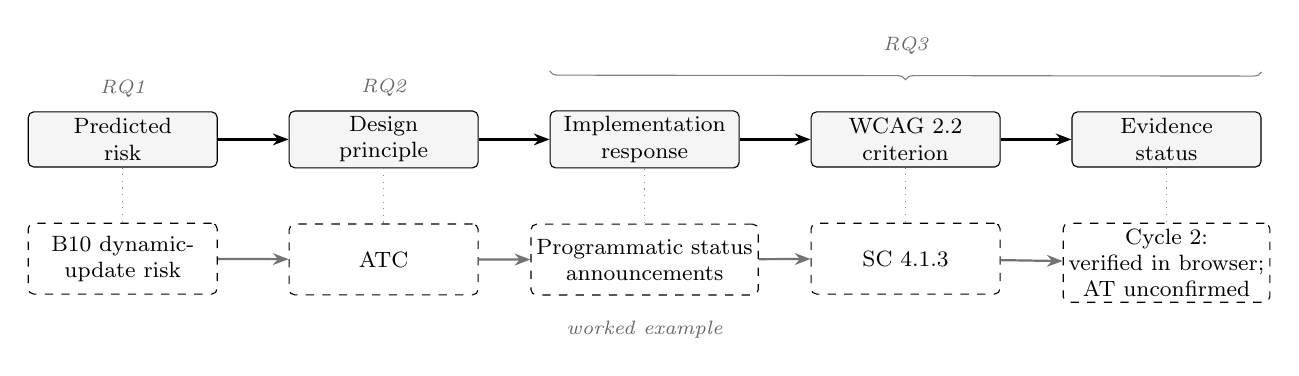
\begin{tikzpicture}[
  font=\footnotesize,
  stage/.style={draw, rounded corners=2pt, minimum height=7mm, minimum width=24mm, align=center, fill=black!4, inner sep=2pt},
  ex/.style={draw, dashed, rounded corners=2pt, minimum height=9mm, minimum width=24mm, align=center, inner sep=2pt},
  ar/.style={-{Stealth[length=2mm]}, thick},
  lbl/.style={font=\scriptsize\itshape, text=black!60}
]
\node[stage] (r) {Predicted\\risk};
\node[stage, right=9mm of r] (p) {Design\\principle};
\node[stage, right=9mm of p] (i) {Implementation\\response};
\node[stage, right=9mm of i] (c) {WCAG~2.2\\criterion};
\node[stage, right=9mm of c] (e) {Evidence\\status};
\foreach \a/\b in {r/p, p/i, i/c, c/e}{\draw[ar] (\a) -- (\b);}
\node[lbl, above=0.5mm of r] {RQ1};
\node[lbl, above=0.5mm of p] {RQ2};
\draw[decorate, decoration={brace, amplitude=3pt}, black!50]
  ([yshift=5mm]e.north east) -- ([yshift=5mm]i.north west)
  node[midway, above=1mm, lbl] {RQ3};
\node[ex, below=7mm of r] (r2) {B10 dynamic-\\update risk};
\node[ex, below=7mm of p] (p2) {ATC};
\node[ex, below=7mm of i] (i2) {Programmatic status\\announcements};
\node[ex, below=7mm of c] (c2) {SC~4.1.3};
\node[ex, below=7mm of e] (e2) {Cycle~2:\\verified in browser;\\AT unconfirmed};
\foreach \a/\b in {r2/p2, p2/i2, i2/c2, c2/e2}{\draw[ar, black!55] (\a) -- (\b);}
\foreach \a/\b in {r/r2, p/p2, i/i2, c/c2, e/e2}{\draw[dotted, black!45] (\a) -- (\b);}
\node[lbl, below=2mm of i2] {worked example};
\end{tikzpicture}
\caption{The BCHAIN-ACCESS traceability chain. Each predicted accessibility risk is traced through its governing design principle, implementation response, criterion-level WCAG~2.2 check, and evidence status; RQ1 and RQ2 concern the first two elements; the brace marks the elements RQ3 adds beyond the principles, which together make the chain auditable. The dashed row traces B10 as a worked example, including the point at which the evidence stops. Table~\ref{tab:traceability} records the complete chain for B1--B12.}
\label{fig:traceability-chain}
\end{figure*}

To keep the framework auditable, each predicted risk is traced through its governing principle, standards or heuristic basis, prototype response or design recommendation, and current evidence status. Fig.~\ref{fig:traceability-chain} shows the structure of this chain and traces one risk through it; Table~\ref{tab:traceability} records it for all twelve risks. Evidence status is cumulative: one response may be standards-derived, implemented, technically tested, expert-inspected, subsequently remediated, and still require target-user confirmation.

The following evidence-status terms are used: \textit{standards-derived}, supported by an identified standard, heuristic, or domain requirement; \textit{implemented}, present in the reference artifact; \textit{simulated}, represented for demonstration but not implemented as a production mechanism; \textit{technically verified}, covered by retained automated, contract, integration, or recorded manual-browser evidence; \textit{expert-inspected}, examined in the Cycle~1 expert assessment; \textit{remediated and technically verified}, changed after evaluation and checked within the retained engineering scope; \textit{not implemented}, retained as a framework recommendation only; and \textit{target-user confirmation required}, indicating that effectiveness remains untested with disabled end users.

\begin{table*}[!t]
\caption{Risk-to-Evidence Traceability in BCHAIN-ACCESS}
\label{tab:traceability}
\centering
\footnotesize
\setlength{\tabcolsep}{3pt}
\renewcommand{\arraystretch}{1.08}
\begin{tabularx}{\textwidth}{p{0.13\textwidth}p{0.075\textwidth}p{0.16\textwidth}X p{0.25\textwidth}}
\toprule
\textbf{Risk Proposition} & \textbf{Principle} & \textbf{Basis} & \textbf{Response or Status} & \textbf{Evidence Status} \\
\midrule
B1 Key-management burden & AAD & H5, H6 & Simulated interface entry; production authentication not implemented & Standards-derived; simulated; expert-inspected; target-user confirmation required \\
B2 Authentication complexity & AAD & SC~2.2.1, SC~3.3.8 & No real authentication workflow evaluated & Standards-derived; simulated only; target-user confirmation required \\
B3 Authentication alternatives & AAD & SC~3.3.8 & Accessible-authentication and representative-access recommendations & Standards-derived; not implemented; target-user confirmation required \\
B4 Unclear status & PTD & H1, SC~4.1.3 & Plain-language transaction and workflow status & Remediated and technically verified: programmatic heading focus and concise transition announcements implemented in the Cycle~2 build; live screen-reader confirmation remains outstanding \\
B5 Technical language & PTD & SC~3.1.3, SC~3.1.5 (AAA) & Inline explanations and plain-language FAQ & Implemented; expert-inspected; target-user confirmation required \\
B6 Opaque permissions & PTD & H2 & Storage, consent, permission, and audit presentation & Implemented; expert-inspected; target-user confirmation required \\
B7 Non-actionable errors & CID & H9, SC~3.3.1 & Plain-language error and recovery guidance & Remediated and technically verified: record-loading, audit-loading, and transaction failures were visibly presented and programmatically announced in the tested error states \\
B8 Inadequate confirmation & CID & H5, SC~3.3.2 & Two-stage review and confirmation & Implemented; technically verified; expert-inspected; target-user confirmation required \\
B9 Limited reversal & CID & H3, SC~3.3.4 & Minimum wait and cancellation until confirmation; later revocation & Implemented; technically verified; expert-inspected; duration requires target-user confirmation \\
B10 Dynamic-update risk & ATC & SC~4.1.3 & Programmatic status announcements & Remediated and technically verified: live-region infrastructure, confirmation availability, success messages, and workflow-transition focus were inspected in the Cycle~2 browser states; assistive-technology compatibility remains unconfirmed \\
B11 Input operability and target size & ATC & SC~2.1.1, SC~2.4.3, SC~2.4.7, SC~2.5.8 & Keyboard path, focus treatment, and target-size adjustments & Remediated and technically verified: principal workflow operability, audit- and revocation-dialog focus containment, focus restoration, and affected minimum target dimensions passed the recorded manual checks \\
B12 Visual distinguishability & ATC & SC~1.4.3, SC~1.4.11 & Contrast checks, non-color status cues, and responsive layout & Remediated and technically verified for reflow: the status panel moves into normal flow at narrow widths and the tested 320-CSS-pixel layout did not reproduce the earlier overlap; complete dynamic-state contrast measurement remains outstanding \\
\bottomrule
\end{tabularx}
\end{table*}

SC~2.2.1 applies when a workflow requires the user to act within a time limit. It is not applied to the implemented minimum wait because no post-wait completion deadline is imposed. Accessible authentication under SC~3.3.8 remains relevant to the simulated authentication workflow and any future production implementation.

\subsection{Three-Part Evidence Review}

BCHAIN-ACCESS organizes evidence collection through three complementary reviews, labelled A--C to distinguish them from the five DSR method stages in Section~\ref{sec:methodology}. Review~A records blockchain-security assumptions, implemented controls, audit status, and residual risks. Review~B records regulatory-awareness considerations, including jurisdiction, governance roles, lawful-basis analysis, rights handling, biometric implications, DPIA status, and applicable standards versions. Review~C records criterion-level accessibility findings, usability observations, assistive-technology configurations, task evidence, and participant boundaries. Each review produces evidence, limitations, unresolved risks, and required follow-up; none produces an automatic compliance, legal, or security verdict.

\section{Framework Operationalization}
\label{sec:operationalization}

This section operationalizes BCHAIN-ACCESS through criterion-level accessibility reporting, a reference smart-contract interface, a structured evidence-recording procedure, and five evidence dimensions used to organize the evaluation results.

\subsection{Criterion-Level Accessibility Evidence}

Accessibility findings are reported by WCAG~2.2 success criterion, applicability, tested interface state, method, Cycle~1 result, and Cycle~2 status. Automated, manual, not-applicable, and not-fully-evaluated results are kept separate. No weighted coverage score or percentage is used as a substitute for criterion-level interpretation.

\subsection{Smart Contract Interface Specification}

\begin{sloppypar}
The reference consent interface contains six functions (\texttt{initiateGrant}, \texttt{confirmGrant}, \texttt{cancelPendingGrant}, \texttt{revokeAccess}, \texttt{checkAccess}, and \texttt{getAuditLog}). The initiate/confirm flow is a two-stage delayed-confirmation state machine, not commit--reveal: no hidden commitment or later secret revelation is used. The implementation enforces a minimum wait before confirmation and permits cancellation until confirmation. Production use would require independent audit, identity and key-management design, privacy engineering, and deployment-specific authorization analysis.
\end{sloppypar}

Two additional contract functions, \texttt{registerRecord} and \texttt{transferOwnership}, support setup and administration. They are included in the final-contract development-network gas measurements reported in Supplementary~S1 but are not part of the six-function consent interface. Supplementary~S1 also reports the measured Cycle~2 logger, gateway-administration, and pause functions.

\subsection{BCHAIN-ACCESS Evidence-Recording Procedure}

Algorithm~\ref{alg:bchain} operationalizes the framework as a structured evidence-recording procedure. It records controls, limitations, unresolved risks, and required follow-up across the three reviews without collapsing the evidence into an aggregate verdict.

\begin{algorithm}
\caption{BCHAIN-ACCESS three-part evidence-recording procedure}
\label{alg:bchain}
\begin{algorithmic}[1]
\Require System $S$ with architecture $A$, interface $I$, documentation $D$
\Ensure Evidence report $R$ with controls, unresolved risks, and follow-up

\State \textbf{Review A --- Blockchain security}
\State Record threat assumptions, implemented controls, audit status, and residual risks

\State \textbf{Review B --- Regulatory awareness}
\State Record jurisdiction, roles, lawful-basis analysis, rights handling, DPIA status, and applicable standards versions

\State \textbf{Review C --- HCI and accessibility}
\State Report criterion-level WCAG results, manual issues, tested states, task evidence, assistive-technology scope, and participant boundary
\State \Return $R$ with evidence status, unresolved risks, and required follow-up
\end{algorithmic}
\end{algorithm}

\subsection{Evaluation Evidence Dimensions}
\label{sec:evidence-dimensions}

The evaluation is organized through five evidence dimensions. These dimensions identify the type and boundary of the evidence collected; they are not thresholds, validation criteria, or compliance benchmarks.

\noindent\textbf{ED1, Criterion-level accessibility evidence:} WCAG~2.2 applicability, tested state, method, automated findings, manual findings, unresolved issues, and remediation status.

\noindent\textbf{ED2, Heuristic and qualitative inspection evidence:} Criterion-linked free-text issues and recommendations. The accompanying coarse heuristic rating distribution is reported in Supplementary~S8.3 but is excluded from the principal results for the reasons given in Section~\ref{subsec:heuristic-evaluation}.

\noindent\textbf{ED3, Expert task-workbook evidence:} Active interaction time and system waiting time, reported descriptively. The task-completion, error, and difficulty fields are reported in Supplementary~S8.4 and excluded from the principal results for the reasons given in Section~\ref{subsec:task-workbook}.

\noindent\textbf{ED4, Perceived-usability evidence:} The SUS score distribution for the expert sample. It is reported in Supplementary~S8.5 and excluded from the principal results, because a perceived-usability score obtained from unblinded evaluators inspecting an artifact built around the principles they were shown cannot support an accessibility or usability claim.

\noindent\textbf{ED5, Post-evaluation questionnaire evidence:} Item-level and participant-level responses from the custom questionnaire. Reported in Supplementary~S8.6 and excluded from the principal results for the reasons given in Section~\ref{subsec:a11y-questionnaire}.

Together, ED1--ED5 organize heterogeneous evidence without collapsing it into a single score or pass/fail verdict.

\section{Reference Artifact and Technical Verification}
\label{sec:implementation}

This section describes the two-component reference artifact used to operationalize BCHAIN-ACCESS and records the evidence available for each component. The artifact comprises an accessibility-oriented user-interface prototype and a separately tested local-EVM consent backend. These components demonstrate framework realizability within a development environment; they are not presented as a production healthcare system.

\subsection{Artifact Components and Evidence Boundaries}

\noindent\textbf{Component 1, user-interface prototype.}
The single-page HTML/CSS/JavaScript interface operationalizes the four BCHAIN-ACCESS principles through a reference-patient consent workflow. It presents record and permission status, provider selection, grant review, delayed confirmation, cancellation, revocation, audit information, and help content. The fingerprint control is a simulated entry mechanism rather than biometric authentication. The Cycle~2 interface communicates directly with the Flask gateway; when the local EVM is unavailable, the gateway explicitly uses its in-memory fallback rather than a separate browser-memory interface.

\noindent\textbf{Component 2, local-EVM reference backend.}
The backend comprises \texttt{HealthAccessControl.sol}, a local Hardhat EVM, and a Flask/Web3.py gateway. The contract supports record registration, grant initiation, delayed confirmation, cancellation, revocation, access checking, audit retrieval, and ownership transfer. An explicit in-memory fallback preserves demonstration behavior when the local EVM is unavailable, but fallback identifiers and EVM transaction hashes remain separately labelled.

\noindent\textbf{Evidence boundary.}
The Cycle~1 ten-expert assessment concerned the interface workflow. Backend behavior was examined separately through contract tests, static analysis, gas profiling, and integration verification. The expert assessment therefore does not provide evidence about contract security, public-network behavior, production identity management, or backend performance.

\begin{table*}[!t]
\caption{Reference-Artifact Components and Evidence Boundaries}
\label{tab:artifact-boundary}
\centering
\footnotesize
\begin{tabularx}{\textwidth}{p{0.16\textwidth}p{0.18\textwidth}p{0.18\textwidth}X}
\toprule
\textbf{Activity} & \textbf{Interface State} & \textbf{Backend State} & \textbf{Evidence Boundary} \\
\midrule
Cycle~1 expert assessment & Integrated evaluation interface & Backend mode by session not logged; local EVM or explicit fallback may have been used & Expert observations and workbook-reported interaction data; session build and environment not archived (L4) \\
Cycle~1 automated reports & Deposited rendered states with varying or partly unknown scope; relationship to a specific session build unverified & Backend and contract not inspected & Tool-specific DOM findings only \\
Cycle~2 integration verification & Integrated Cycle~2 interface & Flask gateway and fresh local Hardhat deployment & Functional grant, confirmation, cancellation, revocation, access-check, and audit paths \\
Cycle~2 automated scan & Cycle~2 initial rendered state & Backend outside scan scope & Initial-state automated evidence only; not a complete-process re-evaluation \\
Cycle~2 engineering verification, 15 July 2026 & Twelve enumerated Cycle~2 states, including both dialogs, three error presentations, FAQ expansion, and narrow-viewport inspection & Cycle~2 contract and gateway source & Live-state accessibility evidence, final 28-test contract result, Slither output, and residual-risk record; no conformance or security-assurance determination \\
\bottomrule
\end{tabularx}
\end{table*}

\begin{figure}[!htbp]
\centering

\includegraphics[width=\linewidth,height=0.72\textheight,keepaspectratio]{images/Figure_1.png}
\caption{Composite interface states in the BCHAIN-ACCESS reference artifact: (A) simulated entry control; (B) record and provider-access presentation; (C) the minimum-wait state before confirmation; and (D) confirmation with a development-ledger transaction identifier.}
\label{fig:prototype-screenshots}
\end{figure}

The detailed implementation-status matrix and the retained Cycle~1 metadata are reported in Supplementary~S9. Representative interface states for the reference artifact are shown in Fig.~\ref{fig:prototype-screenshots}.

\subsection{Local-EVM Consent Backend}
\label{subsec:blockchain-architecture}

The four-layer architecture of BCHAIN-ACCESS is presented in Fig.~\ref{fig:architecture}.

\begin{figure}[!htbp]
\centering
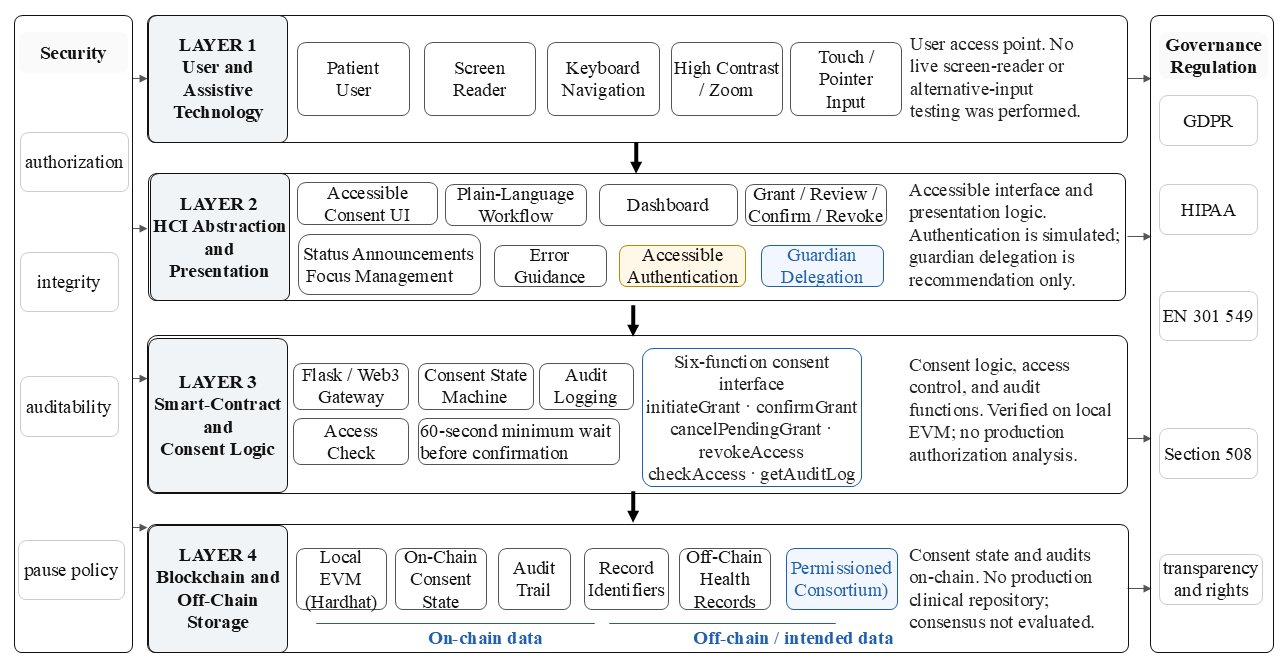
\includegraphics[width=\linewidth,keepaspectratio]{images/Figure_5_architecture_proper_editable.png}
\caption{Implemented and intended boundaries of the BCHAIN-ACCESS reference architecture. The tested artifact includes the HTML interface, Flask gateway, local EVM consent contract, audit structures, and seeded record identifiers; production clinical-record storage, user-controlled wallets, real biometric authentication, live assistive-technology validation, and deployment governance remain outside the demonstrated scope.}
\label{fig:architecture}
\end{figure}

\subsubsection{Consent State Model}

The reference contract implements a patient-controlled consent state model. The record owner may initiate a grant, confirm it after the configured minimum wait, cancel it before confirmation, revoke confirmed access, query current access, and retrieve the contract audit history. The \texttt{onlyPatient} restriction binds these state-changing operations to the record owner in the reference model; it is not a complete organizational identity, role-management, or guardian-delegation system.

Let $P$, $D$, and $R$ denote the sets of patients, providers, and records. Let $\omega_r\in\{0,1\}^{256}$ denote the record identifier supplied to the contract. In a production deployment, this identifier may be derived as $H(\text{record data}\parallel\text{salt})$. The reference artifact instead uses seeded 32-byte identifiers and does not implement clinical-record storage or a salt store. With current timestamp $t$ and minimum pending interval $\Delta = 60$\,s, an access grant is the tuple
\begin{equation}
\label{eq:grant}
G(p,d,\omega_r)=\langle \alpha,\tau_{\text{exp}},\tau_{\text{grant}},\tau_{\text{lock}},\text{active}\rangle,
\end{equation}
where $\alpha$ is the access level (the prototype implements View-Only, $\alpha=1$; the model extends to Download, $\alpha=2$), $\tau_{\text{exp}}$ the expiry ($0$ = infinite), $\tau_{\text{grant}}$ the finalization time, $\tau_{\text{lock}}$ the lock indicator, and $\text{active}$ the status flag. Access is granted only when the grant is active, unlocked, and unexpired:
\begin{equation}
\label{eq:access-check}
\begin{aligned}
\text{Access}(p,d,\omega_r,t)=\text{True}\iff{}&\text{active}\land(\tau_{\text{lock}}=0)\\
&\land(\tau_{\text{exp}}=0\lor t\le\tau_{\text{exp}}).
\end{aligned}
\end{equation}

\begin{figure}[!t]
\centering
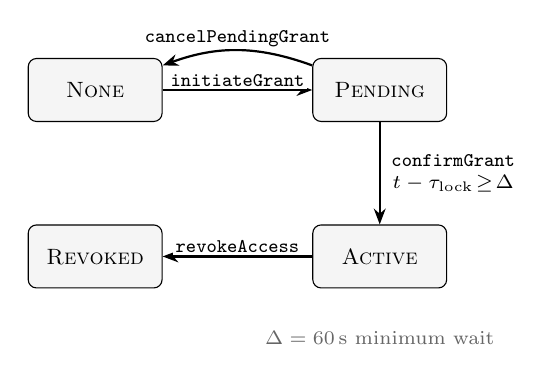
\begin{tikzpicture}[
  font=\footnotesize,
  st/.style={draw, rounded corners=3pt, minimum height=8mm, minimum width=17mm, align=center, fill=black!4},
  ar/.style={-{Stealth[length=2mm]}, thick},
  el/.style={font=\scriptsize, align=center, inner sep=1pt, fill=white}
]
\node[st] (none) {\textsc{None}};
\node[st, right=19mm of none] (pend) {\textsc{Pending}};
\node[st, below=13mm of pend] (act) {\textsc{Active}};
\node[st, left=19mm of act] (rev) {\textsc{Revoked}};
\draw[ar] (none) -- node[el, above]{\texttt{initiateGrant}} (pend);
\draw[ar] (pend) -- node[el, right, xshift=1mm]{\texttt{confirmGrant}\\$t-\tau_{\text{lock}}\!\geq\!\Delta$} (act);
\draw[ar] (act) -- node[el, above]{\texttt{revokeAccess}} (rev);
\draw[ar] (pend) to[out=160, in=20] node[el, above]{\texttt{cancelPendingGrant}} (none);
\node[el, below=4mm of act, text=black!60, yshift=-1mm] {$\Delta=60$\,s minimum wait};
\end{tikzpicture}
\caption{The reference consent state machine. The record owner may initiate a grant, confirm it once the configured minimum wait $\Delta$ has elapsed, cancel it at any point before confirmation, and revoke confirmed access. The initiate/confirm sequence is a two-stage delayed confirmation, not a commit--reveal scheme.}
\label{fig:state-machine}
\end{figure}

The resulting state machine is shown in Fig.~\ref{fig:state-machine}. It enforces a 60-second minimum wait before \texttt{confirmGrant}. In Cycle~2 the contract was changed so that an unconfirmed grant can be cancelled before or after the wait and until confirmation. This control reduces accidental activation but does not guarantee coercion resistance or broader security.

\subsubsection{Gateway and Fallback Behavior}

The Flask/Web3.py gateway builds, signs, and submits transactions to the local EVM using a configured development account. Connected-EVM write failures return an error without advancing the corresponding gateway consent state. EVM transaction hashes and fallback demonstration identifiers are retained separately. When the EVM is unavailable, the gateway may enter an explicitly labelled in-memory demonstration mode; this mode is excluded from blockchain-verification claims.

\subsubsection{Security and Deployment Boundaries}

The backend is a development reference artifact. It uses local development accounts, process-memory state, and development CORS settings and does not implement production key custody, identity proofing, guardian delegation, encrypted clinical-record storage, production gateway authentication, or consortium governance. The Cycle~2 local-EVM contract restricts audit-log submission to the owner or configured authorized gateway; production identity and gateway authentication remain outside scope. The threat--control--residual-risk and STRIDE matrices are provided in Supplementary~S2 and~S4.

\subsubsection{Technical Verification}

The Cycle~2 contract was compiled with solc~0.8.26 and evaluated on Hardhat Chain~ID~1337. The final Hardhat suite contained 28 tests, all of which passed on 15 July 2026. The retained output covers the consent lifecycle, access guards, state and security invariants, authorized and unauthorized audit logging, gateway administration, zero-address rejection, owner and non-owner pause administration, paused grant behavior, continued cancellation and revocation while paused, and operation after unpausing. A fresh deployment exercised record registration, grant initiation, rejection of early confirmation, confirmation after the configured minimum wait, positive access checking, revocation, and negative access checking after revocation. The retained contract audit sequence includes \texttt{RECORD\_REGISTERED}, \texttt{GRANT\_INITIATED}, \texttt{GRANT\_CONFIRMED}, and \texttt{REVOKE}.

Slither~0.11.5 was rerun on the final Cycle~2 contract. The retained output reports six low-severity timestamp-dependence findings associated with the minimum-wait and expiration logic and 35 informational naming-convention findings; it contains no high- or medium-severity detector output. Static analysis does not replace fuzzing, dynamic adversarial analysis, or independent audit.

Final-contract development-network gas measurements, test configuration, static-analysis results, and residual risks are reported in Supplementary~S1, S2, S4, and S6. These results demonstrate the tested local lifecycle and code properties within the recorded development environment.

\subsubsection{Final Cycle~2 Engineering Verification}

Cycle~2 refined the prototype in two passes and produced the artifact that underwent a final researcher-led engineering verification on 15 July 2026 at commit \texttt{360eaa2a26b2f2b4fef98c0667f87db09e5e5120}. The accessibility component evaluated 12 enumerated interface states: landing, dashboard, record selection, review, countdown, confirmation success, audit-dialog open, revocation-dialog open, expanded FAQ, record-loading failure, audit-loading failure, and transaction failure. Standalone axe-core~4.10.0 reports recorded zero violations in these tested states; five states also contained tool-marked incomplete items retained for manual review. Manual browser verification separately examined keyboard operability, dialog focus containment and restoration, wizard-transition focus, target dimensions, error presentation, and narrow-viewport reflow. The three failure presentations were invoked through the verification harness to inspect their rendered and programmatic error states; this was not dynamic RPC failure-injection testing.

Cycle~2 added programmatic focus movement for dashboard and wizard transitions, accessible audit and revocation dialogs with focus trapping and Escape handling, visible and programmatically announced error messages, minimum 24-by-24-CSS-pixel targets for the affected controls, and narrow-viewport repositioning of the blockchain-status panel. These findings describe the tested Cycle~2 states and do not constitute a whole-artifact WCAG conformance determination. The Cycle~2 verification did not include live NVDA, JAWS, or VoiceOver testing.

The smart-contract remediation restricted access-attempt logging to the owner or an authorized gateway, introduced owner-controlled gateway administration, enforced a documented pause policy for grant initiation and confirmation while preserving cancellation and revocation, and restored normal execution after unpausing. The Flask gateway was also changed to accept exactly one record per state-changing request, preventing the previously identified partial multi-record commit condition.

The consolidated record of this verification, including the retained evidence inventory, is provided in Supplementary~S10. The final Hardhat suite reported 28 passing tests and no failures. The retained cases cover authorized and unauthorized audit logging, gateway administration, zero-address rejection, owner and non-owner pause administration, paused grant behavior, continued cancellation and revocation while paused, and operation after unpausing. Slither~0.11.5 reported six low-severity timestamp-dependency findings associated with the intended confirmation-delay and expiration logic and 35 informational naming-convention findings; no high- or medium-severity Slither detector findings were reported.

\begin{table}[!t]
\caption{Implementation and Evidence Status}
\label{tab:implementation-evidence}
\centering
\footnotesize
\setlength{\tabcolsep}{2.5pt}
\begin{tabularx}{\columnwidth}{L L L}
\toprule
\textbf{Element} & \textbf{Implementation} & \textbf{Evidence Status} \\
\midrule
Plain-language consent workflow & Implemented & Expert-inspected \\
Delayed confirmation & Implemented & Contract and integration tested \\
Cancellation before confirmation & Implemented & Contract and integration tested \\
Revocation and access check & Implemented & Contract and integration tested \\
Audit history & Implemented & Local-EVM tested \\
Logger authorization & Implemented & Remediated and contract-tested: submission restricted to the owner or configured authorized gateway \\
Pause policy & Implemented & Remediated and contract-tested: initiation and confirmation blocked while paused; cancellation and revocation remain available \\
Single-record consent API & Implemented & Mitigated and API-verified: state-changing endpoints reject requests unless exactly one record identifier is supplied before submission \\
Accessible authentication & Simulated & Target-user and production testing required \\
Wizard announcements & Remediated after evaluation & Technically verified across the recorded Cycle~2 states; live screen-reader confirmation outstanding \\
Contextual control names & Remediated after evaluation & Technically verified in the Cycle~2 record and revocation states \\
Dialog focus and target-size adjustments & Remediated after evaluation & Technically verified in the recorded manual browser checks \\
Guardian delegation & Not implemented & Framework recommendation \\
Production identity/key management & Not implemented & Deployment engineering required \\
\bottomrule
\end{tabularx}
\end{table}
\section{Exploratory Expert Issue-Identification and Feasibility Assessment}
\label{sec:feasibility}

The exploratory assessment examined whether the BCHAIN-ACCESS principles were represented in the reference interface and whether criterion-linked inspection could identify actionable usability and accessibility issues. The assessment produced six qualitative issues, criterion-level manual findings, a uniform coarse heuristic pattern, workbook-reported task data, SUS responses, and custom-questionnaire responses.

Three streams are reported as results: the Cycle~1 criterion-level manual findings, the free-text observations that yielded the six expert-identified issues, and the elapsed task timings, the last reported descriptively only. Four are excluded: the coarse heuristic ratings (ED2), the completion, error, and difficulty fields (ED3), the SUS scores (ED4), and the custom questionnaire responses (ED5). The excluded material is disclosed in full in Supplementary~S8.3--S8.6, for the reasons set out in Sections~\ref{subsec:heuristic-evaluation}, \ref{subsec:task-workbook}, \ref{subsec:sus}, and~\ref{subsec:a11y-questionnaire}. It is retained for transparency rather than withdrawn, and no claim in this paper rests on it. Fig.~\ref{fig:evidence-funnel} summarizes the disposition of each stream.

\begin{figure*}[!t]
\centering
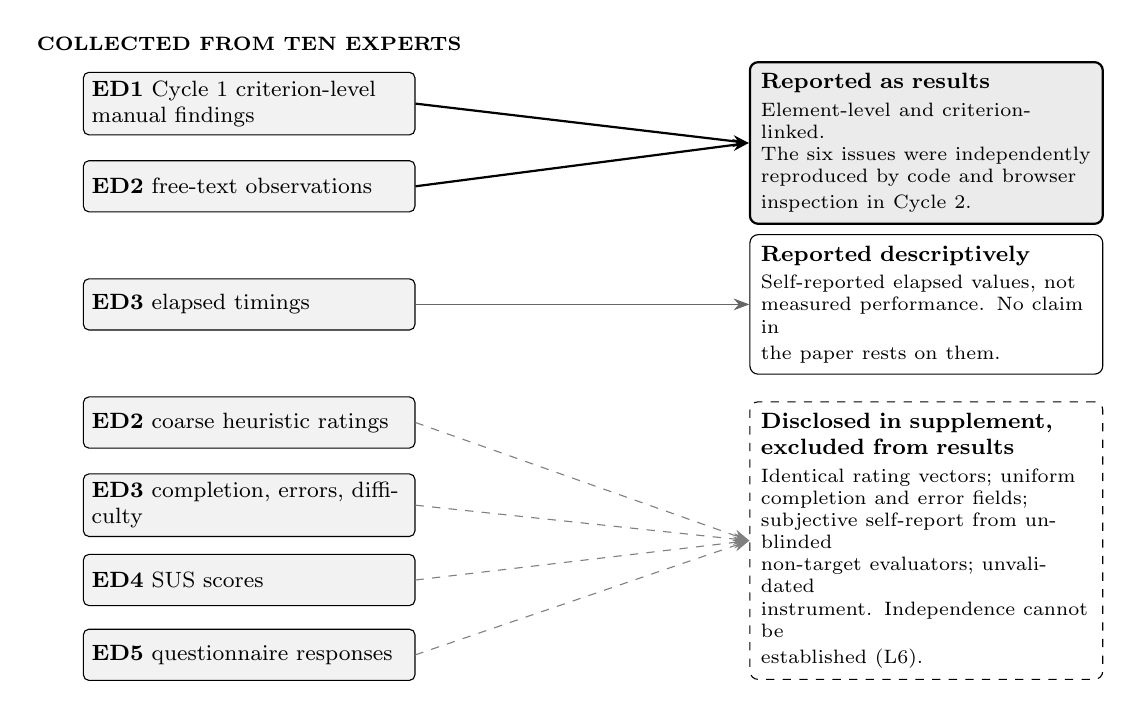
\begin{tikzpicture}[
  font=\footnotesize,
  ed/.style={draw, rounded corners=2pt, minimum height=6.5mm, text width=40mm,
             align=left, fill=black!5, inner sep=3pt},
  keep/.style={draw, thick, rounded corners=3pt, align=left, fill=black!8, inner sep=4pt, text width=42mm},
  desc/.style={draw, rounded corners=3pt, align=left, fill=white, inner sep=4pt, text width=42mm},
  drop/.style={draw, dashed, rounded corners=3pt, align=left, fill=white, inner sep=4pt, text width=42mm},
  ark/.style={-{Stealth[length=2mm]}, thick},
  amid/.style={-{Stealth[length=2mm]}, black!60},
  adr/.style={-{Stealth[length=2mm]}, black!50, dashed}
]
\node[ed] (a1) at (0,0)     {\textbf{ED1} Cycle~1 criterion-level manual findings};
\node[ed] (a2) at (0,-1.05) {\textbf{ED2} free-text observations};
\node[ed] (m1) at (0,-2.55) {\textbf{ED3} elapsed timings};
\node[ed] (b1) at (0,-4.05) {\textbf{ED2} coarse heuristic ratings};
\node[ed] (b2) at (0,-5.10) {\textbf{ED3} completion, errors, difficulty};
\node[ed] (b3) at (0,-6.05) {\textbf{ED4} SUS scores};
\node[ed] (b4) at (0,-7.00) {\textbf{ED5} questionnaire responses};
\node[font=\scriptsize\bfseries, above=1.5mm of a1] {COLLECTED FROM TEN EXPERTS};
\node[keep] (rep) at (8.6,-0.5) {\textbf{Reported as results}\\[2pt]
  {\scriptsize Element-level and criterion-linked.\\The six issues were independently\\reproduced by code and browser\\inspection in Cycle~2.}};
\node[desc] (dsc) at (8.6,-2.55) {\textbf{Reported descriptively}\\[2pt]
  {\scriptsize Self-reported elapsed values, not\\measured performance. No claim in\\the paper rests on them.}};
\node[drop] (exc) at (8.6,-5.55) {\textbf{Disclosed in supplement,\\excluded from results}\\[2pt]
  {\scriptsize Identical rating vectors; uniform\\completion and error fields;\\subjective self-report from unblinded\\non-target evaluators; unvalidated\\instrument. Independence cannot be\\established (L6).}};
\draw[ark] (a1.east) -- (rep.west);
\draw[ark] (a2.east) -- (rep.west);
\draw[amid] (m1.east) -- (dsc.west);
\draw[adr] (b1.east) -- (exc.west);
\draw[adr] (b2.east) -- (exc.west);
\draw[adr] (b3.east) -- (exc.west);
\draw[adr] (b4.east) -- (exc.west);
\end{tikzpicture}
\caption{Disposition of the expert-study evidence. Two streams are reported as results; one is reported descriptively but supports no claim; four are disclosed in full in the supplement and excluded, because they cannot be shown to rest on independent observations of the artifact by target users (Limitation~L6). ED2 and ED3 each produced streams in more than one category. Cycle~2 engineering verification is reported separately and is not part of this figure.}
\label{fig:evidence-funnel}
\end{figure*}


Ten domain experts completed the unblinded, asynchronous protocol. They were not recruited as disabled end-user participants, and disability status was not collected. The assessment therefore addresses expert issue identification and reference-interface feasibility rather than target-user accessibility effectiveness.

\subsection{Study Design}
\label{subsec:study-design}

The assessment was organized through ED1--ED5: criterion-level accessibility evidence, heuristic and qualitative observations, task-workbook evidence, perceived usability, and custom-questionnaire evidence.

The assessment was designed as a convergent mixed-methods study\cite{creswell2017research}, combining automated inspection of retained rendered states, criterion-level expert review, Nielsen heuristic inspection, an eight-task expert walkthrough, SUS, and a custom post-evaluation questionnaire. What is reported, however, is not a convergent design: the quantitative strands did not survive the evidence assessment described below and are excluded, so the results presented are the criterion-level and qualitative strands only. Evidence sources were analyzed descriptively and retained separately rather than collapsed into a single accessibility or usability score.

\subsection{Participants and Procedure}
\label{subsec:participants}

Ten domain experts completed the protocol remotely and asynchronously using the same evaluation packet. The packet contained the interface link, eight workflow tasks, Nielsen heuristic sheet, criterion-level accessibility checklist, SUS, and custom questionnaire. Evaluators submitted responses independently and could not inspect one another's submissions. They were not blinded to BCHAIN-ACCESS or to the fact that the interface had been designed around the inspected principles.

Participation was voluntary. Before beginning the assessment, evaluators received information about the study purpose, procedures, data handling, confidentiality, and their right to withdraw without penalty. Each evaluator provided documented consent through WhatsApp. Records were pseudonymized as E1--E10 and results are reported in aggregate. The consent messages are retained privately because they contain identifying information. No formal institutional ethics-committee approval, exemption, or determination that formal review was unnecessary was obtained; this is reported as a study limitation.

The retained evaluator summary records professional backgrounds spanning accessibility, UX/HCI, frontend engineering, digital health, occupational therapy, and assistive technology, with five to ten years of reported experience. Evaluators used their own environments, which were not specified, standardized, or recorded; one evaluator's comments indicate unversioned NVDA use during the session. The study therefore did not include a specified or reproducible assistive-technology test condition, and no screen-reader evidence from these sessions is treated as an assistive-technology compatibility result. Expertise labels and credential strings were not independently verified and are therefore treated as descriptive metadata. Full evaluator-level information is provided in Supplementary~S8.2.

% Declared before the result subsections so this retained main-text table can occupy
% the next two-column float position without forcing the smaller detail tables to stack.
\begin{table*}[!t]
\centering
\caption{Expert-Identified Issues and Anticipated Interaction Implications}
\label{tab:expert-issues}
\small
\renewcommand{\arraystretch}{1.12}
\begin{tabularx}{\textwidth}{|P{4.0cm}|L|L|P{1.5cm}|}
\hline
\textbf{Issue} & \textbf{Anticipated Interaction Implication} & \textbf{Response or Follow-Up} & \textbf{Source} \\
\hline
Mandatory 60-second minimum wait & The wait may create unnecessary delay or frustration; its adequacy for different interaction needs is unestablished & Empirically evaluate the duration and whether a shorter or user-selectable safety delay is preferable & E7, E9 \\
\hline
Step transitions in the grant wizard are not announced via ARIA live region & Screen-reader users may not perceive that the step has changed (Step~1$\rightarrow$Step~2) & Announce each step change through an ARIA live region & E6, E10 \\
\hline
``Remove Access'' button lacks provider context in its accessible name & Screen-reader users hear only ``Remove Access'' without knowing which provider it targets & Set the accessible name to ``Remove access for [provider]'' & E10 \\
\hline
Record title and metadata are not clearly separated for screen readers & Title and date are announced as a single string, reducing clarity & Use semantic markup to separate title from metadata & E10 \\
\hline
Small accordion controls / touch targets in the FAQ & Users with motor impairments or switch access may find repeated activation inefficient & Enlarge targets; make the full question header activatable; add an ``expand all'' option & E9, E10 \\
\hline
High text density on the Review page & Users with cognitive or reading difficulties may be overloaded & Offer a simplified-summary mode and plainer vocabulary & E9 \\
\hline
\end{tabularx}
\tablenote{\textit{Note.} Issues are drawn from retained evaluator comments. Anticipated implications are analytical interpretations used to guide remediation and future evaluation; they are not participant-confirmed effects.}
\end{table*}

\subsection{ED1: Automated and Criterion-Level Accessibility Evidence}
\label{subsec:auto-evaluation}

The deposited automated artifacts include two Lighthouse~13.4.0 reports, one WAVE report, an undated limited axe-core summary, a dated axe-core~4.12.1 initial-state report, an intermediate live axe-core~4.8.2 dialog inspection, and the final standalone axe-core~4.10.0 state reports. These artifacts differ in date, tool version, URL, retained scope, and remediation stage and are therefore reported separately rather than aggregated. The 15 July Cycle~2 initial state produced zero axe-core violations. The intermediate 15 July dialog inspection reported one moderate \texttt{region} finding. After the corresponding dialog remediation, the final state-by-state verification retained 12 reports with zero violations; five reports also contain tool-marked incomplete items requiring manual review. Manual keyboard, focus, dialog, target-size, error-presentation, and reflow checks are recorded separately. Cycle~1 manual criterion-level findings remain unchanged. The artifact-by-artifact automated summary and complete WCAG~2.2 A/AA matrix are reported in Supplementary~S5. Fig.~\ref{fig:wcag-coverage} shows the Cycle~1 result recorded for every criterion in that matrix.
\begin{figure*}[!t]
\centering
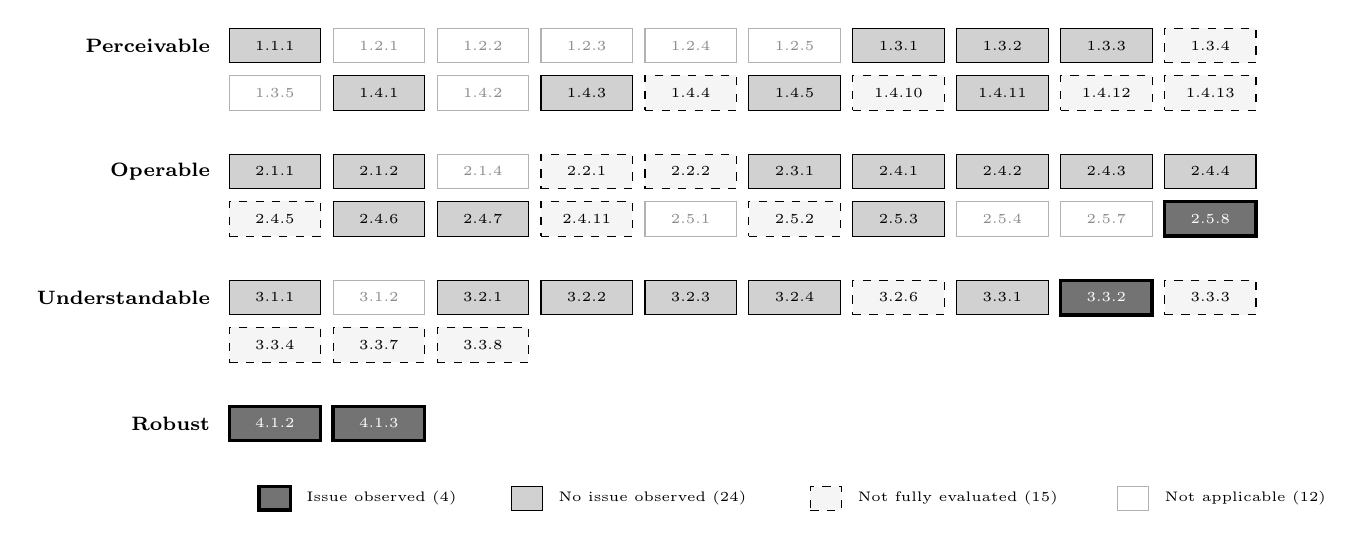
\begin{tikzpicture}[
  font=\scriptsize,
  cell/.style={draw, minimum width=11.6mm, minimum height=4.4mm, inner sep=0pt, font=\tiny},
  issue/.style={fill=black!55, text=white, very thick},
  noissue/.style={fill=black!18},
  partial/.style={fill=black!4, dashed},
  na/.style={fill=white, draw=black!30, text=black!45},
  glabel/.style={anchor=east, font=\scriptsize\bfseries},
  leg/.style={draw, minimum width=4mm, minimum height=3mm, inner sep=0pt}
]
\node[glabel] at (-0.7,0.00) {Perceivable};
\node[cell, noissue] at (0.00,0.00) {1.1.1};
\node[cell, na] at (1.32,0.00) {1.2.1};
\node[cell, na] at (2.64,0.00) {1.2.2};
\node[cell, na] at (3.96,0.00) {1.2.3};
\node[cell, na] at (5.28,0.00) {1.2.4};
\node[cell, na] at (6.60,0.00) {1.2.5};
\node[cell, noissue] at (7.92,0.00) {1.3.1};
\node[cell, noissue] at (9.24,0.00) {1.3.2};
\node[cell, noissue] at (10.56,0.00) {1.3.3};
\node[cell, partial] at (11.88,0.00) {1.3.4};
\node[cell, na] at (0.00,-0.60) {1.3.5};
\node[cell, noissue] at (1.32,-0.60) {1.4.1};
\node[cell, na] at (2.64,-0.60) {1.4.2};
\node[cell, noissue] at (3.96,-0.60) {1.4.3};
\node[cell, partial] at (5.28,-0.60) {1.4.4};
\node[cell, noissue] at (6.60,-0.60) {1.4.5};
\node[cell, partial] at (7.92,-0.60) {1.4.10};
\node[cell, noissue] at (9.24,-0.60) {1.4.11};
\node[cell, partial] at (10.56,-0.60) {1.4.12};
\node[cell, partial] at (11.88,-0.60) {1.4.13};
\node[glabel] at (-0.7,-1.60) {Operable};
\node[cell, noissue] at (0.00,-1.60) {2.1.1};
\node[cell, noissue] at (1.32,-1.60) {2.1.2};
\node[cell, na] at (2.64,-1.60) {2.1.4};
\node[cell, partial] at (3.96,-1.60) {2.2.1};
\node[cell, partial] at (5.28,-1.60) {2.2.2};
\node[cell, noissue] at (6.60,-1.60) {2.3.1};
\node[cell, noissue] at (7.92,-1.60) {2.4.1};
\node[cell, noissue] at (9.24,-1.60) {2.4.2};
\node[cell, noissue] at (10.56,-1.60) {2.4.3};
\node[cell, noissue] at (11.88,-1.60) {2.4.4};
\node[cell, partial] at (0.00,-2.20) {2.4.5};
\node[cell, noissue] at (1.32,-2.20) {2.4.6};
\node[cell, noissue] at (2.64,-2.20) {2.4.7};
\node[cell, partial] at (3.96,-2.20) {2.4.11};
\node[cell, na] at (5.28,-2.20) {2.5.1};
\node[cell, partial] at (6.60,-2.20) {2.5.2};
\node[cell, noissue] at (7.92,-2.20) {2.5.3};
\node[cell, na] at (9.24,-2.20) {2.5.4};
\node[cell, na] at (10.56,-2.20) {2.5.7};
\node[cell, issue] at (11.88,-2.20) {2.5.8};
\node[glabel] at (-0.7,-3.20) {Understandable};
\node[cell, noissue] at (0.00,-3.20) {3.1.1};
\node[cell, na] at (1.32,-3.20) {3.1.2};
\node[cell, noissue] at (2.64,-3.20) {3.2.1};
\node[cell, noissue] at (3.96,-3.20) {3.2.2};
\node[cell, noissue] at (5.28,-3.20) {3.2.3};
\node[cell, noissue] at (6.60,-3.20) {3.2.4};
\node[cell, partial] at (7.92,-3.20) {3.2.6};
\node[cell, noissue] at (9.24,-3.20) {3.3.1};
\node[cell, issue] at (10.56,-3.20) {3.3.2};
\node[cell, partial] at (11.88,-3.20) {3.3.3};
\node[cell, partial] at (0.00,-3.80) {3.3.4};
\node[cell, partial] at (1.32,-3.80) {3.3.7};
\node[cell, partial] at (2.64,-3.80) {3.3.8};
\node[glabel] at (-0.7,-4.80) {Robust};
\node[cell, issue] at (0.00,-4.80) {4.1.2};
\node[cell, issue] at (1.32,-4.80) {4.1.3};
\node[leg, issue]   at (0.00,-5.75) {};
\node[anchor=west, font=\tiny] at (0.28,-5.75) {Issue observed (4)};
\node[leg, noissue] at (3.20,-5.75) {};
\node[anchor=west, font=\tiny] at (3.48,-5.75) {No issue observed (24)};
\node[leg, partial] at (7.00,-5.75) {};
\node[anchor=west, font=\tiny] at (7.28,-5.75) {Not fully evaluated (15)};
\node[leg, na]      at (10.90,-5.75) {};
\node[anchor=west, font=\tiny] at (11.18,-5.75) {Not applicable (12)};
\end{tikzpicture}
\caption{Cycle~1 evidence coverage for the 55 WCAG~2.2 Level~A/AA criteria; obsolete SC~4.1.1 is excluded. Shading reports bounded evidence, not conformance: 15 criteria were not fully evaluated. Supplementary~S5 gives the state, method, and Cycle~2 status for every criterion.}
\label{fig:wcag-coverage}
\end{figure*}

\subsection{ED2: Heuristic and Qualitative Inspection Evidence}
\label{subsec:heuristic-evaluation}

All ten evaluators assigned H1--H8 and H10 a rating of 0 and H9 a rating of 1. Every evaluator therefore returned an identical ten-item rating vector; the per-evaluator matrix is reproduced without alteration in Supplementary~S8.3.

We do not report these ratings as a result. A coarse scale can be expected to compress responses toward a common value, but scale coarseness does not account for exact agreement across ten independently administered evaluators on all ten dimensions. The retained records cannot distinguish among the candidate explanations. The evaluation packet may have constrained the response effectively to a single admissible pattern; the submissions may not have been independent despite the asynchronous protocol; or the consolidated workbook may not preserve the responses as originally supplied. No administration log, timestamp, submission record, or original response document survives that would allow these to be separated. Because the ratings cannot be shown to be ten independent observations, they cannot function as evidence about the artifact, and no chance-corrected agreement coefficient is meaningful for a degenerate distribution in any case.

The free-text observations recorded in the same packet are treated differently. They vary across evaluators, are attributable to identified evaluators, are specific to interface elements, and were independently reproduced by later code and browser inspection during remediation. They are reported in Section~\ref{subsec:expert-issues} as the principal expert result on that basis rather than on the basis of the rating instrument.

A finer post-hoc re-rating was summarized after the original responses were inspected, but its scale anchors, instructions, timing, and participant-level matrix were not preserved. It is likewise excluded.

\subsection{ED3: Expert Task-Workbook Evidence}
\label{subsec:task-workbook}

The eight scripted tasks covered interface entry, record viewing, access inspection, grant initiation, confirmation review, confirmation after the minimum wait, revocation, and help-content access. Tasks were completed in a fixed order.

The retained task CSV contains evaluator identifier, task identifier, active interaction time, error count, difficulty rating, and notes. It does not contain row-level completion, assistance, restart, incomplete-attempt, timestamp, or telemetry fields, and no observer record, screen recording, or interaction log was kept. The per-task values are reproduced in Supplementary~S8.4.

The completion and error fields are excluded from the principal results. The consolidated workbook reports completion of every scripted task row and a mean error count of 0.0 for all ten evaluators, but ``error'' is not operationally defined beyond the numeric field, and nothing in the retained package can distinguish an evaluator who made no errors from one who recorded none. Together with the identical heuristic vectors discussed in Section~\ref{subsec:heuristic-evaluation}, these fields cannot be treated as ten independent observations, and no claim here rests on them (L6).

The self-reported difficulty ratings are excluded on the same grounds as ED4: difficulty is a subjective evaluative judgment supplied by the same unblinded evaluators, and it is not distinguishable from a perceived-usability response in what it can support. The ratings are reported in Supplementary~S8.4.

The elapsed timings are retained descriptively, because they record how long an action took rather than an evaluator's opinion of the artifact. Mean active interaction time across the eight tasks was 9.7 seconds ($SD=5.9$). Task~T6 (confirmation after the minimum wait) recorded the longest mean active time at 17.3 seconds; because the 60-second system wait was timed separately and excluded from that figure, the minimum elapsed duration for T6 was approximately 77.3 seconds. These remain self-reported workbook values rather than measured performance, and no claim in this paper rests on them.

The workflow operationalizes the hypothetical consent scenario introduced in Section~V; the complete step-by-step mapping is provided in Supplementary~S8.7.

\subsection{Expert-Identified Issues and Anticipated Interaction Implications}
\label{subsec:expert-issues}

Free-text observations identified six issues that aggregate scores obscured (Table~\ref{tab:expert-issues}). They are retained as the principal expert-study result because they provide concrete inspection and follow-up targets.

The criterion-level and free-text instruments are two views of one set of findings, not two independent sets. Four of the six issues correspond to recorded Level~A/AA criterion failures and appear in the Supplementary~S5 matrix as issues observed against SC~4.1.3, SC~4.1.2, SC~3.3.2, and SC~2.5.8. The remaining two correspond to no Level~A/AA success criterion at all: the mandatory minimum wait is an interaction-design choice rather than a failure under SC~2.2.1, and plain-language presentation is addressed only at Level~AAA (SC~3.1.5), which is outside the instrument. Criterion-level conformance checking alone would not have surfaced either. This is the practical case for pairing criterion-level review with qualitative inspection instead of treating conformance checking as sufficient, and it is the clearest evidence this study provides for separating evidence types rather than aggregating them.

Issue identification was concentrated: all six issues came from four evaluators (E6, E7, E9, and E10), and the remaining six evaluators recorded no retained issues. Uneven issue identification across individual evaluators is an expected property of heuristic inspection~\cite{nielsen1992finding}, but it means the expert layer of this study rests on four contributors rather than ten, which further narrows what it establishes.

The qualitative issues are not downgraded by the uniform coarse heuristic rating or the workbook-reported completion values. They remain criterion-linked evidence requiring remediation, retesting, or target-user confirmation.

\FloatBarrier
\subsection{ED4: Perceived Usability}
\label{subsec:sus}

After completing the walkthrough, evaluators completed the standard ten-item SUS\cite{brooke1996sus}. The scores, the per-evaluator distribution, and the scoring procedure are reported in Supplementary~S8.5.

The result is excluded from the principal findings. The evaluators were unblinded, knew that the interface had been constructed around the principles they were inspecting, and were not recruited as users of the workflow. A favourable perceived-usability score under those conditions is consistent with the artifact being usable and equally consistent with demand characteristics, and the design cannot separate the two. Reporting the score in the main text would lend quantitative weight to a measure that carries no evidential weight for either the accessibility claims or the usability claims of this paper.

\subsection{ED5: Custom Questionnaire Evidence}
\label{subsec:a11y-questionnaire}

The custom ten-item questionnaire covered navigation, instructions, keyboard access, contrast, error messages, perceived control, independent-use comfort, error recovery, comprehension, and responsiveness. Responses and item-level results are reported in Supplementary~S8.6.

This instrument is also excluded from the principal results. It was completed by the same ten unblinded evaluators, in the same session, under the same demand characteristics that exclude ED4, and it has the additional weakness of being author-designed with no reliability or validity evidence. An unvalidated instrument administered to non-target users who knew the design intent cannot measure accessibility, and reporting its mean alongside that caveat would lend it a weight the design cannot support.

\subsection{Evidence Synthesis}
\label{subsec:discussion-results}

\begin{table*}[!t]
\caption{Evaluation Evidence Dimensions and Boundaries}
\label{tab:evidence-dimensions-results}
\centering
\footnotesize
\renewcommand{\arraystretch}{1.08}
\begin{tabularx}{\textwidth}{p{0.08\textwidth}p{0.22\textwidth}X X}
\toprule
\textbf{ID} & \textbf{Evidence Dimension} & \textbf{Principal Finding} & \textbf{Evidence Boundary} \\
\midrule
ED1 & Criterion-level accessibility and Cycle~2 technical evidence & Cycle~1 criterion-level inspection recorded issues against SC~4.1.3 (status announcement), SC~4.1.2 and SC~3.3.2 (contextual name, semantic separation), and SC~2.5.8 (target size). Cycle~2 subsequently addressed the selected implementation issues; state-by-state axe-core reports recorded zero violations across 12 tested states, and manual verification passed the recorded keyboard, focus, dialog, target-size, error-state, and reflow checks & Cycle~1 findings relate to the Cycle~1 artifact; the later results relate only to Cycle~2. No specified or reproducible assistive-technology test condition in Cycle~1 and no live screen-reader testing in the Cycle~2 verification; no disabled-participant evaluation and no whole-artifact WCAG conformance determination \\
ED2 & Heuristic and qualitative inspection & Six actionable qualitative issues retained as the principal expert result & Coarse ratings excluded: identical vectors across all ten evaluators cannot be shown to be independent observations (S8.3); post-hoc re-rating also excluded \\
ED3 & Expert task-workbook evidence & Elapsed timings reported descriptively: mean active task time 9.7 seconds, T6 17.3 seconds plus the separately timed 60-second wait & Completion, error, and difficulty fields excluded (uniform or subjective self-report; ``error'' undefined); no row-level completion field, telemetry, observer record, or session recording \\
ED4 & Perceived usability & Not reported as a finding; scores disclosed in S8.5 & Excluded: unblinded evaluators inspecting a principle-derived artifact; demand characteristics not separable from the measure \\
ED5 & Custom questionnaire evidence & Not reported as a finding; responses disclosed in S8.6 & Excluded: author-designed instrument, reliability and validity not evaluated, administered to the same unblinded non-target evaluators as ED4 \\
\bottomrule
\end{tabularx}
\end{table*}

The evidence sources provide markedly unequal support, and the paper's claims rest on the strongest of them only. ED1 and the retained qualitative observations offer the actionable findings, because they identify criterion-linked interface issues and concrete remediation targets that were subsequently reproduced by code and browser inspection. ED3 contributes descriptive timings only; its completion and error fields are excluded on the same grounds as ED2, and no session record exists against which the workbook values could be checked. ED2, ED4, and ED5 are excluded from the principal results and retained in full in the supplement for transparency. What the expert study contributes is therefore narrow and specific: it identified six actionable, element-level issues that were independently reproduced by code and browser inspection in Cycle~2. That is the claim the design supports, and the paper makes no other claim from it.

The Cycle~1 findings were retained unchanged and used to guide Cycle~2. The Cycle~2 build addressed the selected announcement, accessible-name, dialog, focus-management, target-size, error-presentation, audit-authorization, pause-policy, and multi-record consistency issues. State-by-state interface verification, 28 passing contract tests, and static analysis confirmed the listed corrections within the recorded engineering scope. This evidence describes the Cycle~2 artifact and does not alter the Cycle~1 results. The mandatory wait remains an empirically unresolved interaction-design choice rather than a failure under SC~2.2.1.



%============================================================================
% End of Section IX: Exploratory Expert Issue-Identification and Feasibility Assessment
%============================================================================
%============================================================================
% SECTION X: DISCUSSION, LIMITATIONS, AND FUTURE WORK
% ============================================================
\section{Discussion, Limitations, and Future Work}
\label{sec:discussion}

\subsection{Answers to the Research Questions}

\noindent\textbf{RQ1: Predicted accessibility risks.}
The study formulated twelve standards-informed accessibility-risk propositions across authentication complexity, interface transparency, feedback adequacy, and assistive-technology compatibility. These propositions synthesize accessibility criteria, HCI principles, closely related research, and documentation-based evidence. They identify design risks requiring implementation and evaluation attention; they do not represent participant-confirmed barriers or demonstrated failures in the three illustrative systems.

\noindent\textbf{RQ2: Accessibility-oriented design principles.}
The twelve propositions were translated into four principles: Abstracted Authentication Design, Progressive Transparency Design, Confirmatory Interaction Design, and Assistive-Technology Compatibility. The principles convert broad accessibility and usability concerns into implementable obligations concerning authentication, transparency, confirmation, recovery, feedback, input operability, visual presentation, and programmatic status communication. Their grouping is an author-developed design structure whose adequacy remains open to target-user refinement.

\noindent\textbf{RQ3: Evidence-aware traceability.}
BCHAIN-ACCESS traces each predicted risk to its governing principle, standards basis, implementation response or recommendation, criterion-level check, and evidence status. The framework distinguishes standards-derived requirements, implemented and simulated features, technically verified behavior, expert-inspected issues, Cycle~2 refinement, unresolved risks, and elements requiring target-user confirmation. Its principal contribution is therefore an auditable risk--principle--response--criterion--evidence chain rather than a certification or aggregate accessibility score.

\subsection{Implications for Research and Practice}

\noindent\textbf{Research implications.}
BCHAIN-ACCESS demonstrates how accessibility requirements can be incorporated into Design Science as traceable design obligations rather than added only as post-implementation checks. The evidence-status dimension is particularly important because standards derivation, implementation, automated testing, expert inspection, remediation, and target-user evaluation provide different kinds of support. Retaining these distinctions prevents positive automated scores or expert perceptions from obscuring unresolved manual findings. This study is itself an instance of that mechanism. The expert sample returned favourable perceived-usability and questionnaire responses and recorded no task errors, and under a conventional reporting model those aggregates would have been presented alongside the six unresolved manual findings, lending the artifact an appearance of validation that the design does not support. Applying the evidence-status discipline to our own data required excluding them: they were produced by unblinded non-target evaluators and, in the case of the heuristic ratings, cannot be shown to be independent observations at all. What survives is smaller than the aggregate would have implied and better supported than it: six element-level findings, each reproduced independently by code and browser inspection in Cycle~2. We report this reflexively because a framework that only disciplines other people's evidence would not be worth proposing.

The study also shows that blockchain consent introduces interaction questions that are not resolved by conventional accessibility checking alone. Immutability constrains recovery, delayed finalization complicates status communication, wallet-based authentication can impose cognitive and dexterity demands, and off-chain/on-chain architectures require comprehensible explanations of storage and permission state. These concerns motivate further work at the intersection of accessible interaction design, consent governance, and distributed-system behavior.

\noindent\textbf{Practice implications.}
Development teams can use the BCHAIN-ACCESS traceability structure to record why an accessibility response is required, whether it has been implemented, what evidence supports it, and what remains unresolved. Priority areas include accessible authentication, actionable transaction states, cancellable confirmation, contextual control names, programmatic announcements, keyboard and focus behavior, target size, contrast, error recovery, and understandable permission histories.

Teams should also avoid treating architectural choices as accessibility or compliance guarantees. Off-chain storage does not by itself establish legal compliance; biometrics and representative access introduce privacy, capacity, authorization, and abuse considerations; and a delayed-confirmation mechanism may reduce accidental activation without preventing coercion or guaranteeing usability.

\subsection{Limitations and Threats to Validity}

\noindent\textbf{L1, Documentation-based comparison.}
The three illustrative systems were examined through publications, product material, user reviews, and prior reports rather than direct interaction with preserved live deployments. The resulting evidence codes cannot establish product-level conformance, task impact, frequency, persistence, or severity. Pre-consensus records required to calculate reviewer agreement were not preserved.

\noindent\textbf{L2, No target-user evaluation.}
Evaluators were not recruited as disabled end-user participants, and disability status was not collected. Expert inspection can identify criterion-linked issues but cannot establish lived usability, accessibility effectiveness, comprehension, independence, or acceptability for disabled users.

\noindent\textbf{L3, Limited system sample.}
The documentation review covered three purposively selected systems representing different blockchain-healthcare contexts. The resulting propositions may support analytical transfer to similar interfaces, but their prevalence and applicability across the wider field remain unestablished.

\noindent\textbf{L4, Cycle~1 artifact provenance.}
The Cycle~1 build was not archived before it was refined, so its exact commit, per-session backend mode, session dates, and evaluator environment matrix are not recoverable. The retained Cycle~1 automated reports are dated 29~June and 12~July 2026 and therefore place the cycle before the 15~July Cycle~2 verification, but they are not linked to a specific session build. Cycle~1 and Cycle~2 evidence are consequently reported separately throughout, and no Cycle~2 result is used to characterize the artifact the experts evaluated.

\noindent\textbf{L5, Targeted narrative evidence gathering.}
The related-work synthesis was conducted by one reviewer to support problem formulation and contribution positioning. It was not designed as a systematic, scoping, bibliometric, or exhaustive review; no field-wide prevalence or comprehensive-coverage inference is made.

\noindent\textbf{L6, Unblinded assessment and non-independent quantitative responses.}
The expert assessment was unblinded. All ten evaluators returned identical heuristic rating vectors, reported zero errors on every task, and reported completion of every scripted task. These distributions are not explained by scale coarseness or by an easy artifact: exact agreement across ten independently administered instruments on all ten heuristic dimensions is not a plausible outcome of independent rating, and the retained records contain no administration log, timestamp, submission artifact, or observer sheet that would establish independence. We therefore treat every quantitative expert measure (ED2, ED4, ED5, and the ED3 completion, error, and difficulty fields) as unable to support inference about the artifact, and we exclude them from the principal results rather than reporting them with caveats. The free-text observations are retained because they vary across evaluators, are element-specific, and were independently reproduced during code and browser inspection. This limitation constrains the expert study to issue identification; it provides no measurement of usability, accessibility, or task performance.

\noindent\textbf{L7, Task and questionnaire evidence.}
Task measures were retained through evaluator workbooks rather than observer records, screen recordings, or automatic telemetry. Row-level completion, assistance, restart, and incomplete-attempt fields were not preserved, so the reported timings cannot be independently checked and are presented descriptively only. The SUS and custom-questionnaire responses are excluded from the results under L6 and are retained in the supplement for transparency; the custom instrument additionally has no reliability or validity evidence.

\noindent\textbf{L8, Cycle~2 accessibility-verification scope.}
The Cycle~2 artifact underwent state-by-state axe-core inspection across 12 enumerated interface states together with manual browser checks of keyboard operation, focus containment and restoration, dialog behavior, affected target dimensions, visible error states, and narrow-viewport reflow. Lighthouse was also executed on the Cycle~2 initial state. However, the Cycle~2 verification did not include live NVDA, JAWS, VoiceOver, alternative-input, or disabled-participant evaluation, and the retained checks do not constitute a complete whole-artifact WCAG conformance determination. The earlier expert sessions were conducted in unrecorded evaluator-chosen environments and included unversioned NVDA use by one evaluator; because the configuration, method, and output were not preserved, this does not constitute reproducible screen-reader evidence for any success criterion.

\noindent\textbf{L9, Development-network and security-assurance scope.}
The final local-EVM build restricted audit-log submission, enforced the documented administrative pause policy, and rejected multi-record state-changing API requests before transaction submission. These contract controls were exercised in the final 28-test suite, while the single-record API boundary was verified separately. Nevertheless, the evidence was generated on a single local Hardhat development node using development accounts and in-memory application state. Property-based fuzzing, failure injection under dynamic RPC loss, dynamic adversarial testing, multi-node deployment, production identity and key management, secure clinical-data persistence, and independent smart-contract audit remain outside scope.

\noindent\textbf{L10, Ethics-review provenance.}
Evaluators voluntarily participated after providing documented consent through WhatsApp and were informed that they could withdraw at any time without penalty. Evaluation records were pseudonymized as E1--E10 and reported only in aggregate; no health, biometric, disability-status, or other special-category personal data were collected. No formal institutional ethics-committee approval, exemption, or determination that formal review was unnecessary was obtained. These safeguards do not replace an institutional ethics determination, and its absence may affect eligibility under some publication-venue policies.

\subsection{Future Research}
\label{sec:future-work}

\noindent\textbf{Target-user confirmation and framework refinement.}
The next empirical phase should evaluate and refine BCHAIN-ACCESS with disabled participants and assistive-technology users. The study protocol should be co-designed with relevant community contributors before formal ethics review and preregistration \cite{nosek2018preregistration}. Zhou et al.~\cite{zhou2023accessible} provide a directly applicable precedent for recruiting and evaluating with blind participants in a blockchain interface context. Participants should use their own assistive technologies where feasible, and the evaluation should examine grant initiation, review, cancellation, confirmation, revocation, permission comprehension, transaction-state understanding, accessible authentication, contextual control naming, programmatic announcements, and the acceptability of the confirmation delay. Outcomes should include independent task success, assistance events, comprehension, perceived control, accessibility issues, and qualitative recommendations. Sampling, compensation, eligibility, and analysis procedures should be determined through co-design and feasibility assessment rather than fixed in the present paper.

\noindent\textbf{Artifact and engineering verification.}
Further accessibility research should conduct reproducible live testing with NVDA and VoiceOver, alternative-input technologies, and disabled participants, including evaluation of announcement quality, comprehension, independence, and the acceptability of the mandatory confirmation delay. Further engineering work should add property-based fuzzing, dynamic failure-injection and adversarial tests, multi-node permissioned-network evaluation, production identity and key management, durable encrypted off-chain storage, dependency maintenance, and independent smart-contract audit before any production use. The Cycle~2 artifact and evidence should be deposited as a new versioned archival release identified as the Cycle~2 build.

% ============================================================
% SECTION XI: CONCLUSION
% ============================================================
\section{Conclusion}
\label{sec:conclusion}

This paper presented BCHAIN-ACCESS, a standards-informed and evidence-aware framework for accessibility-oriented blockchain healthcare consent interfaces. The framework translates twelve predicted accessibility-risk propositions into four design principles and connects them to implementation responses, criterion-level WCAG~2.2 checks, and explicit evidence status. Its primary contribution is an auditable risk--principle--response--criterion--evidence traceability structure that distinguishes requirements, implementation, technical verification, expert inspection, remediation, unresolved risks, and future target-user confirmation.

A reference user-interface prototype and separately tested local-EVM backend demonstrated framework operationalization within a development environment. Cycle~1 criterion-level expert inspection identified actionable issues involving wizard-state announcements, contextual control names, target size, semantic presentation, and content density, while the mandatory confirmation wait remained an empirically unresolved usability choice. A second design cycle addressed selected interface, contract, and backend issues identified in the first, and verified the refined artifact across 12 enumerated interface states, a 28-test Hardhat suite, and Slither static analysis. The Cycle~2 build added accessible dialog behavior, programmatic workflow focus, user-visible error states, corrected interactive targets, authorized audit logging, a safety-preserving pause policy, and single-record state-change enforcement. The final standalone axe-core reports recorded zero violations across the 12 tested states; five reports contained incomplete items retained for manual review. All 28 contract tests passed.

These results strengthen the technical feasibility evidence but do not establish whole-artifact WCAG conformance, accessibility effectiveness for disabled users, production security, or independent assurance. BCHAIN-ACCESS nevertheless provides a reusable foundation for making accessibility obligations and evidence boundaries explicit during the design and evaluation of blockchain-mediated healthcare consent. Subsequent work should add live assistive-technology, alternative-input, property-based, failure-injection, and adversarial backend testing and evaluate BCHAIN-ACCESS through co-designed studies involving disabled people and assistive-technology users.

% ============================================================
% BIBLIOGRAPHY
% ============================================================
\bibliographystyle{IEEEtran}
\bibliography{ref_revised}

\end{document}
